
\documentclass{article}
\usepackage{graphicx}
\usepackage{subfig}
\usepackage{amsmath}
\usepackage{float}
\usepackage{booktabs}
\usepackage[margin=1in]{geometry}

\title{CS776 Assignment 3}
\author{Neal Ramaswamy \quad \texttt{nramaswamy@unr.edu}}
\date{October 2025}

\begin{document}

\maketitle

\section{Introduction}

\subsection{Purpose}
The purpose of this assignment is to solve three problems:
\begin{itemize}
    \item Floorplanning
    \item Black-box Function
    \item Traveling Salesman Problem using Genetic Algorithms (GAs)
\end{itemize}

\section{Floorplanning}
\subsection{Problem Statement}
The objective is to determine the optimal dimensions (length and width) of each room in a rectangular apartment floorplan such that total \emph{cost} is minimized while satisfying geometric and proportional constraints.

Each room is assumed rectangular; total apartment cost is the sum of room costs. Cost is area for all rooms except \textbf{Kitchen} and \textbf{Bath}, whose costs are twice their areas. The design must satisfy the dimensional and proportional limits in Table~\ref{tab:floorplan_constraints}. Additionally, there must be a \textbf{3.0-unit-wide space} for a doorway between \textit{Bedroom 2}, \textit{Bedroom 3}, and the \textit{Hall}. The whole floorplan is rectangular.

\begin{table}[H]
\centering
\caption{Room dimension and proportion constraints}
\label{tab:floorplan_constraints}
\begin{tabular}{|c|c|c|c|c|c|c|}
\hline
\textbf{Room} & \textbf{Len (Min)} & \textbf{Len (Max)} & \textbf{Wid (Min)} & \textbf{Wid (Max)} & \textbf{Range} & \textbf{Proportion} \\ \hline
Living  & 8  & 20  & 8  & 20  & 120--300 & 1.5 \\ \hline
Kitchen & 6  & 18  & 6  & 18  & 50--120  & Any \\ \hline
Bath    & 5.5 & 5.5 & 8.5 & 8.5 & ---      & Any \\ \hline
Hall    & 5.5 & 5.5 & 3.5 & 6   & 19--72   & Any \\ \hline
Bed 1   & 10 & 17  & 10 & 17  & 100--180 & 1.5 \\ \hline
Bed 2   & 9  & 20  & 9  & 20  & 100--180 & 1.5 \\ \hline
Bed 3   & 8  & 18  & 8  & 18  & 100--180 & 1.5 \\ \hline
\end{tabular}
\end{table}

\noindent\textbf{Decision variables:} per-room length and width and placement. \quad
\textbf{Objective:} minimize total apartment cost. \quad
\textbf{Constraints:} satisfy Table~\ref{tab:floorplan_constraints}, the 3.0-unit doorway, rectangular rooms and outer boundary.

\subsection{Representation \& Encoding}
Each candidate solution (\emph{chromosome}) encodes one rectangular layout as a vector of seven \texttt{Room} structs:
\[
\texttt{Room} = (\text{length}, \text{width}, \text{x}, \text{y})
\]
for \{\textit{Living, Kitchen, Bath, Hall, Bed1, Bed2, Bed3}\}. Areas are $\text{length}\times\text{width}$. A \texttt{RoomSpec} table (bounds, area ranges, aspect target if any, cost multiplier) mirrors Table~\ref{tab:floorplan_constraints}. Cost multipliers implement Kitchen/Bath at $2\times$ area.

\subsection{Encoding Precision and Decoding}
\paragraph{Chromosome and precision.}
We use a real-coded representation. Each room contributes four genes $(\text{len},\text{wid},x,y)$; the chromosome length is $7\times4=28$ reals. Unless otherwise stated, genes are maintained at two-decimal precision (grid size $0.01$).

\paragraph{Ranges.}
Length/width genes are clamped to their per-room bounds in Table~\ref{tab:floorplan_constraints}; $(x,y)$ are bounded by a conservative enclosing rectangle computed from the sum of minimum areas and aspect constraints.

\paragraph{Decoding.}
A chromosome decodes to axis-aligned rectangles at $(x,y)$ with $(\text{len},\text{wid})$. We do not repair infeasibility; instead, violations (out-of-bounds, overlap, doorway clearance, aspect tolerance) are translated to additive penalties $\Pi(\mathbf{x})$ (Section~\ref{sec:penalties}). The optimizer minimizes $C(\mathbf{x})+\Pi(\mathbf{x})$.

\subsection{Assumptions and Their Relationship to Encoding}
The following modeling assumptions render the problem tractable; each constrains the encoding and/or the penalty function.
\begin{enumerate}
    \item \textbf{Rectangular geometry} for all rooms and the outer boundary. \emph{Encoding:} axis-aligned $(\text{len},\text{wid})$ and placement; overlap checks are AABB.
    \item \textbf{Fixed set of seven named rooms}; topology/adjacency is not optimized. \emph{Encoding:} fixed vector; no slicing tree.
    \item \textbf{Bathroom dimensions fixed}. \emph{Encoding:} bath genes are constants (or hard-clamped).
    \item \textbf{Additive cost} with Kitchen and Bath weighted by $2\times$. \emph{Objective:} independent room areas with multipliers.
    \item \textbf{3.0-unit doorway link} (Bed2, Bed3, Hall). \emph{Penalty:} geometric clearance constraint.
    \item \textbf{Feasibility via penalties} rather than repair. \emph{Search:} infeasible individuals allowed; penalties drive feasibility.
\end{enumerate}

\subsection{Objective Function}
We minimize total cost:
\[
\min\; C(\mathbf{x})=\sum_{r \in \mathcal{R}} \big(\text{mult}_r \cdot \text{area}_r \big)
\]
For feasible solutions, this is the sum of areas with Kitchen/Bath doubled. A theoretical lower bound from per-room minima prints as ``Theoretical Min cost: 632.5'' (tight only if all constraints were jointly attainable).

\subsection{Reporting Conventions (Cost vs.\ Fitness)}
\textbf{We minimize cost.} Optimization is performed on
\[
C(\mathbf{x}) = \sum_{r \in \mathcal{R}} \big(\text{mult}_r \cdot \text{area}_r \big) + \Pi(\mathbf{x}),
\]
where $\Pi(\mathbf{x})$ aggregates penalties. Lower is better.

\paragraph{Caveat on terminology.}
If a value is not confined to $0$--$100$, treat it as \emph{cost}. Only use \emph{fitness} for a $0$--$100$ normalized score for maximization, e.g.,
\[
\mathrm{fitness}(\mathbf{x}) = 100 \cdot \frac{C_{\max} - C(\mathbf{x})}{C_{\max} - C_{\min}}\,.
\]

\paragraph{Practical guidance.}
Label unbounded values as \textbf{cost} (lower is better); use \textbf{fitness} only when normalized; never mix scales on one axis.

\subsection{Constraint Handling (Penalty Method)}\label{sec:penalties}
Violations are penalized additively:
\begin{itemize}
    \item \textbf{Dimensional bounds:} large penalty ($\sim10^3$) per out-of-range length/width.
    \item \textbf{Area range:} medium penalty ($\sim5\cdot10^2$) per violation.
    \item \textbf{Aspect ratio (if specified):} tolerance $\pm0.1$; otherwise penalty ($\sim3\cdot10^2$).
    \item \textbf{Doorway constraint:} enforce $3.0$-unit passage; add penalty on violation.
    \item \textbf{Global rectangularity:} overlap or spillover penalized.
\end{itemize}
Net objective: $C_{\mathrm{eff}}(\mathbf{x}) = C(\mathbf{x}) + \Pi(\mathbf{x})$ (minimize). Feasible $\Leftrightarrow \Pi(\mathbf{x})=0$.

\subsection{Initialization}
Initial population samples per-room $(\text{len},\text{wid})$ within bounds; placements $(x,y)$ in a sufficiently large bounding rectangle. Infeasible individuals are allowed.

\subsection{Selection, Crossover, Mutation, Elitism}
\begin{itemize}
    \item \textbf{Selection:} tournament ($k{=}7$).
    \item \textbf{Crossover:} $p_c{=}0.85$; exchange subsets of room genes (dims+placement).
    \item \textbf{Mutation:} $p_m{=}0.02$ per offspring; jitter dims/placement.
    \item \textbf{Elitism:} top $10$ lowest-cost copied unchanged.
\end{itemize}

\subsection{Parameters \& Runtime Settings}
\begin{center}
\begin{tabular}{ll}
Population size & 200 \\
Generations     & 2000 \\
Crossover rate  & 0.85 \\
Mutation rate   & 0.02 \\
Tournament size & 7 \\
Elite count     & 10 \\
Seed            & 1 \\
\end{tabular}
\end{center}

\subsection{Parameter Exploration}
Three major configurations were evaluated before converging on the final settings.
\begin{table}[H]
\centering
\caption{Parameter exploration for floorplanning GA}
\label{tab:floorplan_params}
\begin{tabular}{lrrrr}
\toprule
Config & Population & Generations & Mutation & Best Cost \\
\midrule
A & 100 & 1000 & 0.01 & 893.2 \\
B & 200 & 2000 & 0.02 & 790.9 \\
C & 300 & 3000 & 0.03 & 788.7 \\
\bottomrule
\end{tabular}
\end{table}

\subsection{Convergence Behavior}
Representative checkpoints (Best \textbar{} Avg Cost):
\begin{verbatim}
Gen  1:  Best Cost 2530.70 | Avg Cost 90851.03
Gen 20:  Best Cost 1337.41 | Avg Cost  7010.13
Gen 100: Best Cost 1045.38 | Avg Cost  8606.21
Gen 200: Best Cost  885.80 | Avg Cost  8843.34
Gen 500: Best Cost  810.36 | Avg Cost  8666.31
Gen 1000: Best Cost  795.19 | Avg Cost  5610.09
Gen 1500: Best Cost  793.53 | Avg Cost  7880.73
Gen 2000: Best Cost  790.96 | Avg Cost  8691.64
\end{verbatim}

\begin{figure}[H]
    \centering
    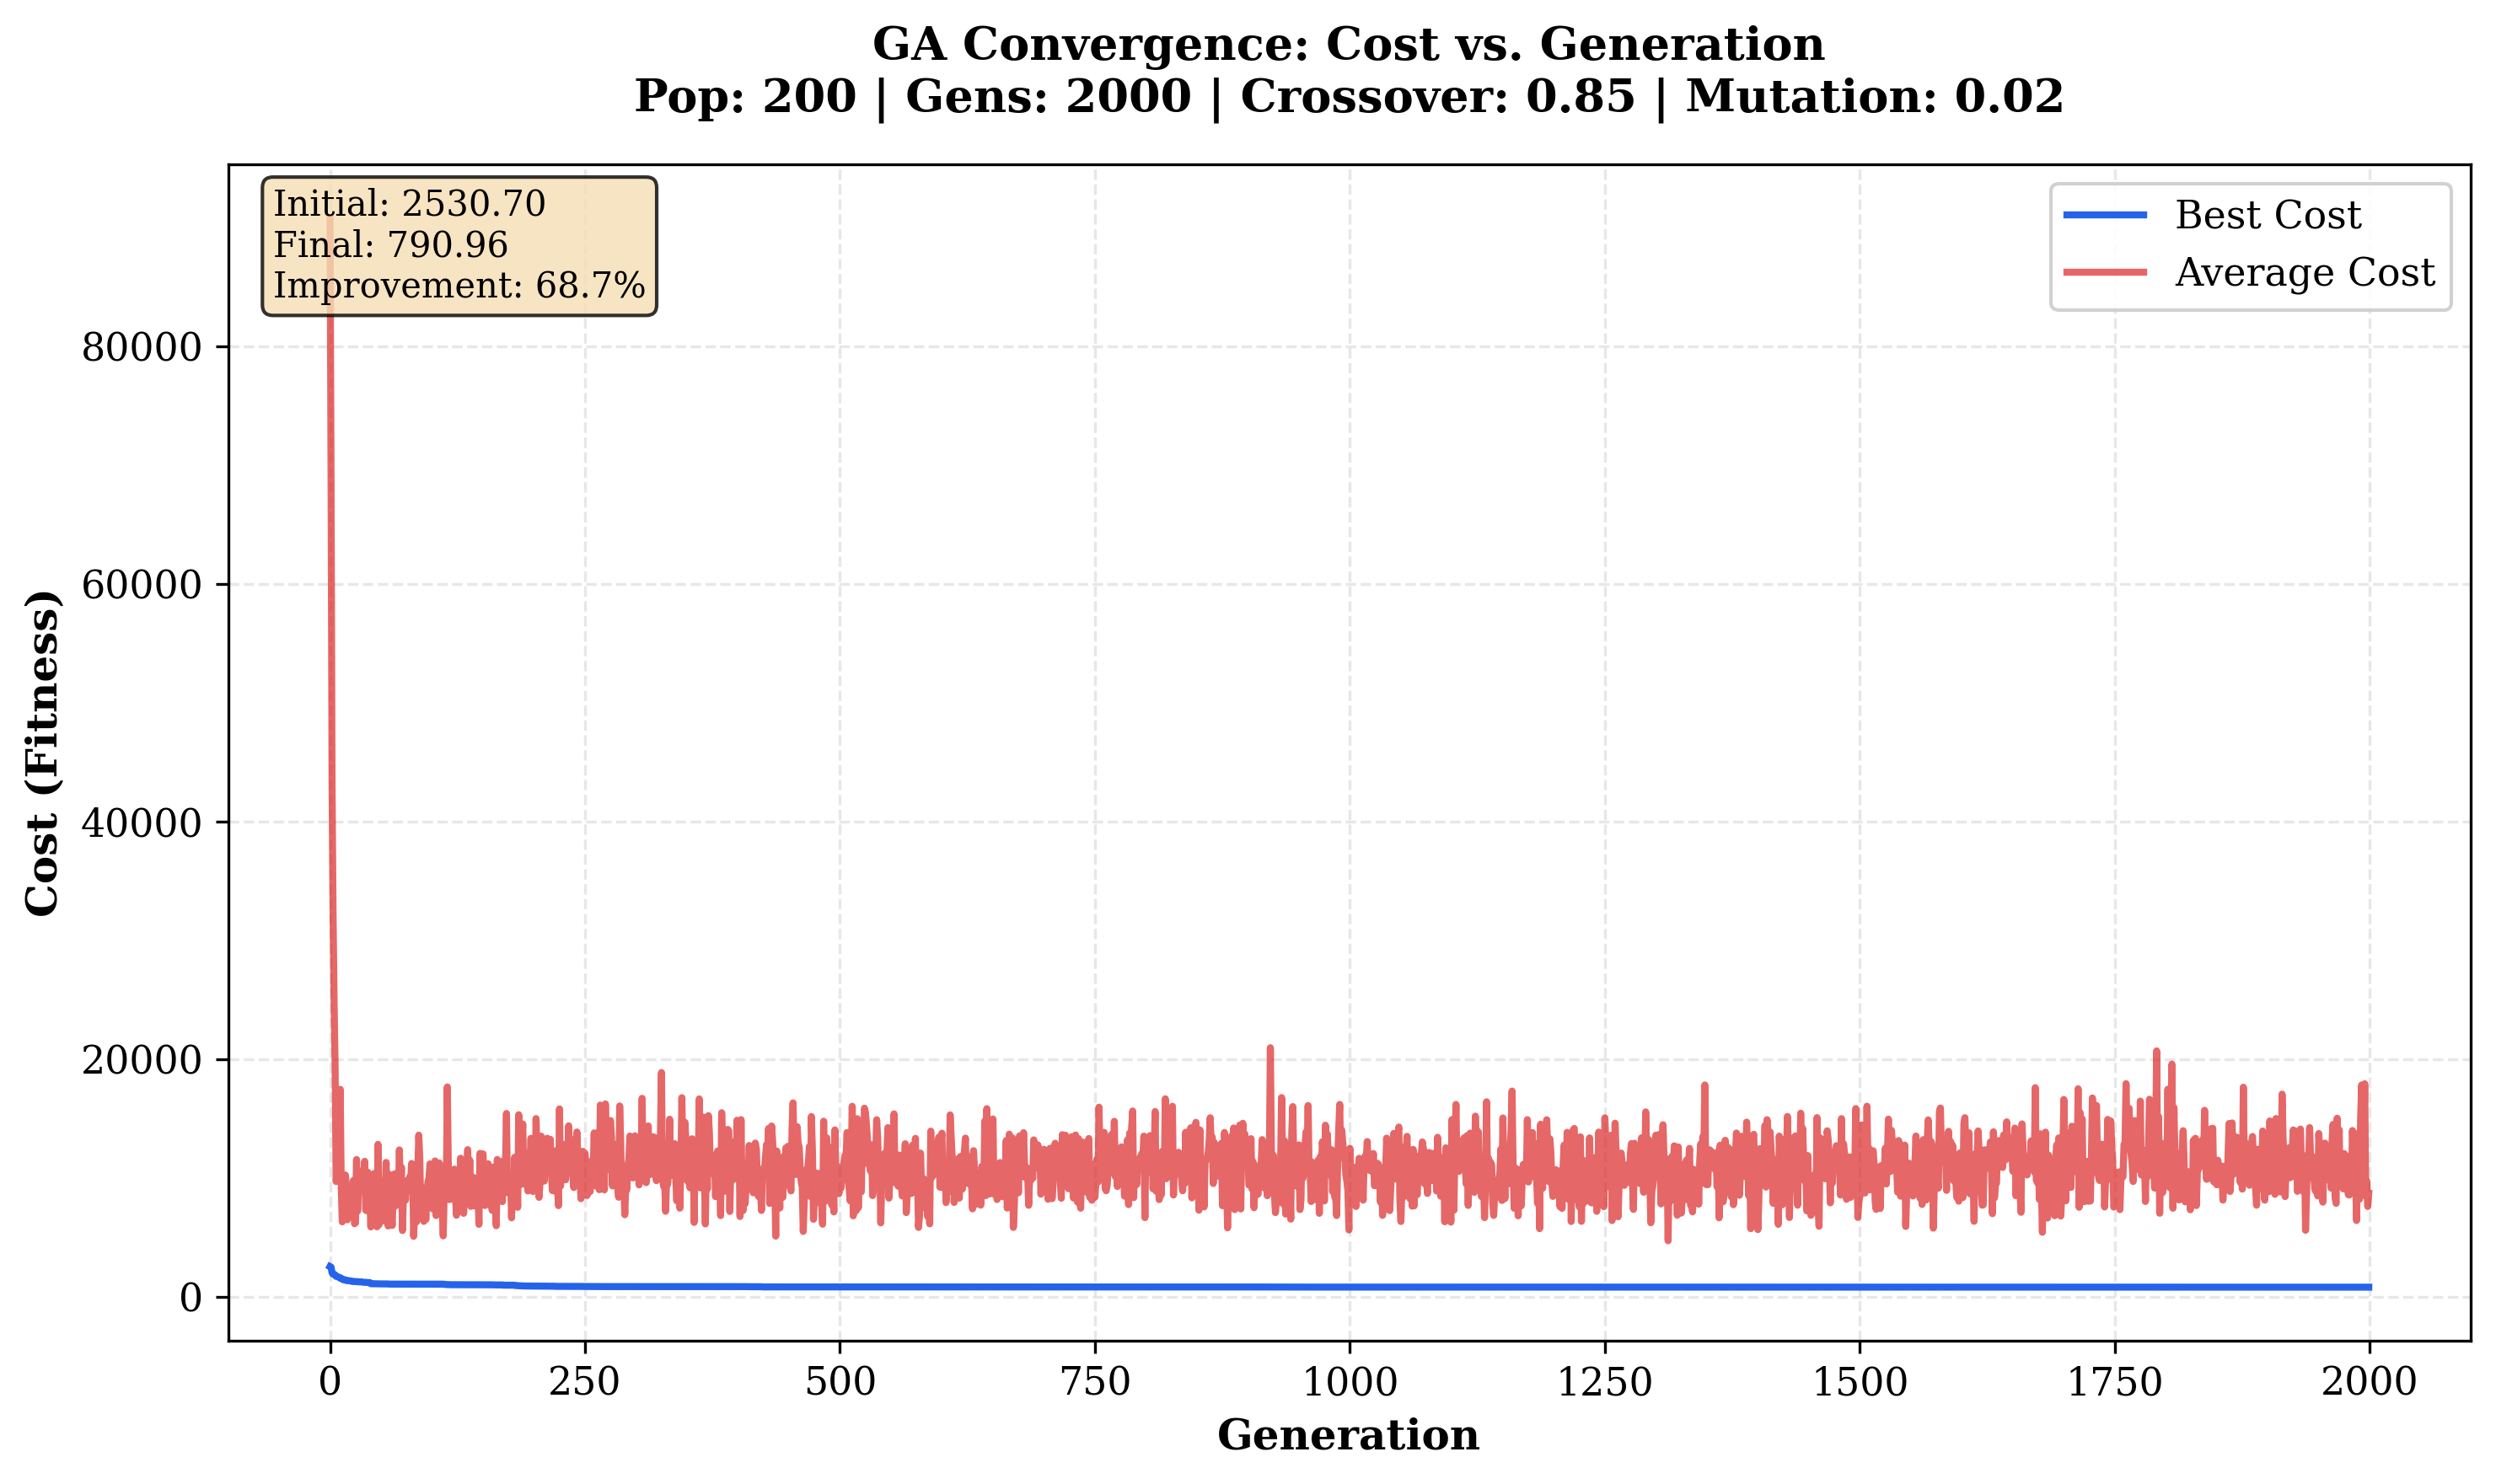
\includegraphics[width=0.8\textwidth]{ga_convergence.png}
    \caption{GA convergence for floorplanning (Best and Average Cost vs.\ Generation).}
\end{figure}

\subsection{Best Solution Found}
At termination, a feasible layout with cost $790.96$ and raw cost $699.84$ (penalty $=0$):
\begin{center}
\begin{tabular}{lrrrrr}
\toprule
Room & Length & Width & Area & X & Y \\
\midrule
Living  & 13.08 &  9.33 & 122.02 & 15.92 & 11.14 \\
Kitchen &  7.96 &  6.28 &  50.02 & 26.03 & 14.23 \\
Bath    &  5.50 &  8.50 &  46.75 &  6.68 & 11.33 \\
Hall    &  3.50 &  5.82 &  20.38 &  7.92 & 33.27 \\
Bed1    & 14.99 & 10.02 & 150.11 &  5.55 & 17.57 \\
Bed2    & 12.60 &  9.00 & 113.42 & 15.58 & 24.22 \\
Bed3    & 12.55 &  8.00 & 100.37 & 24.58 & 24.26 \\
\midrule
\multicolumn{6}{r}{Total Area: 603.07 \qquad Total Cost: 699.84} \\
\bottomrule
\end{tabular}
\end{center}

\begin{figure}[H]
    \centering
    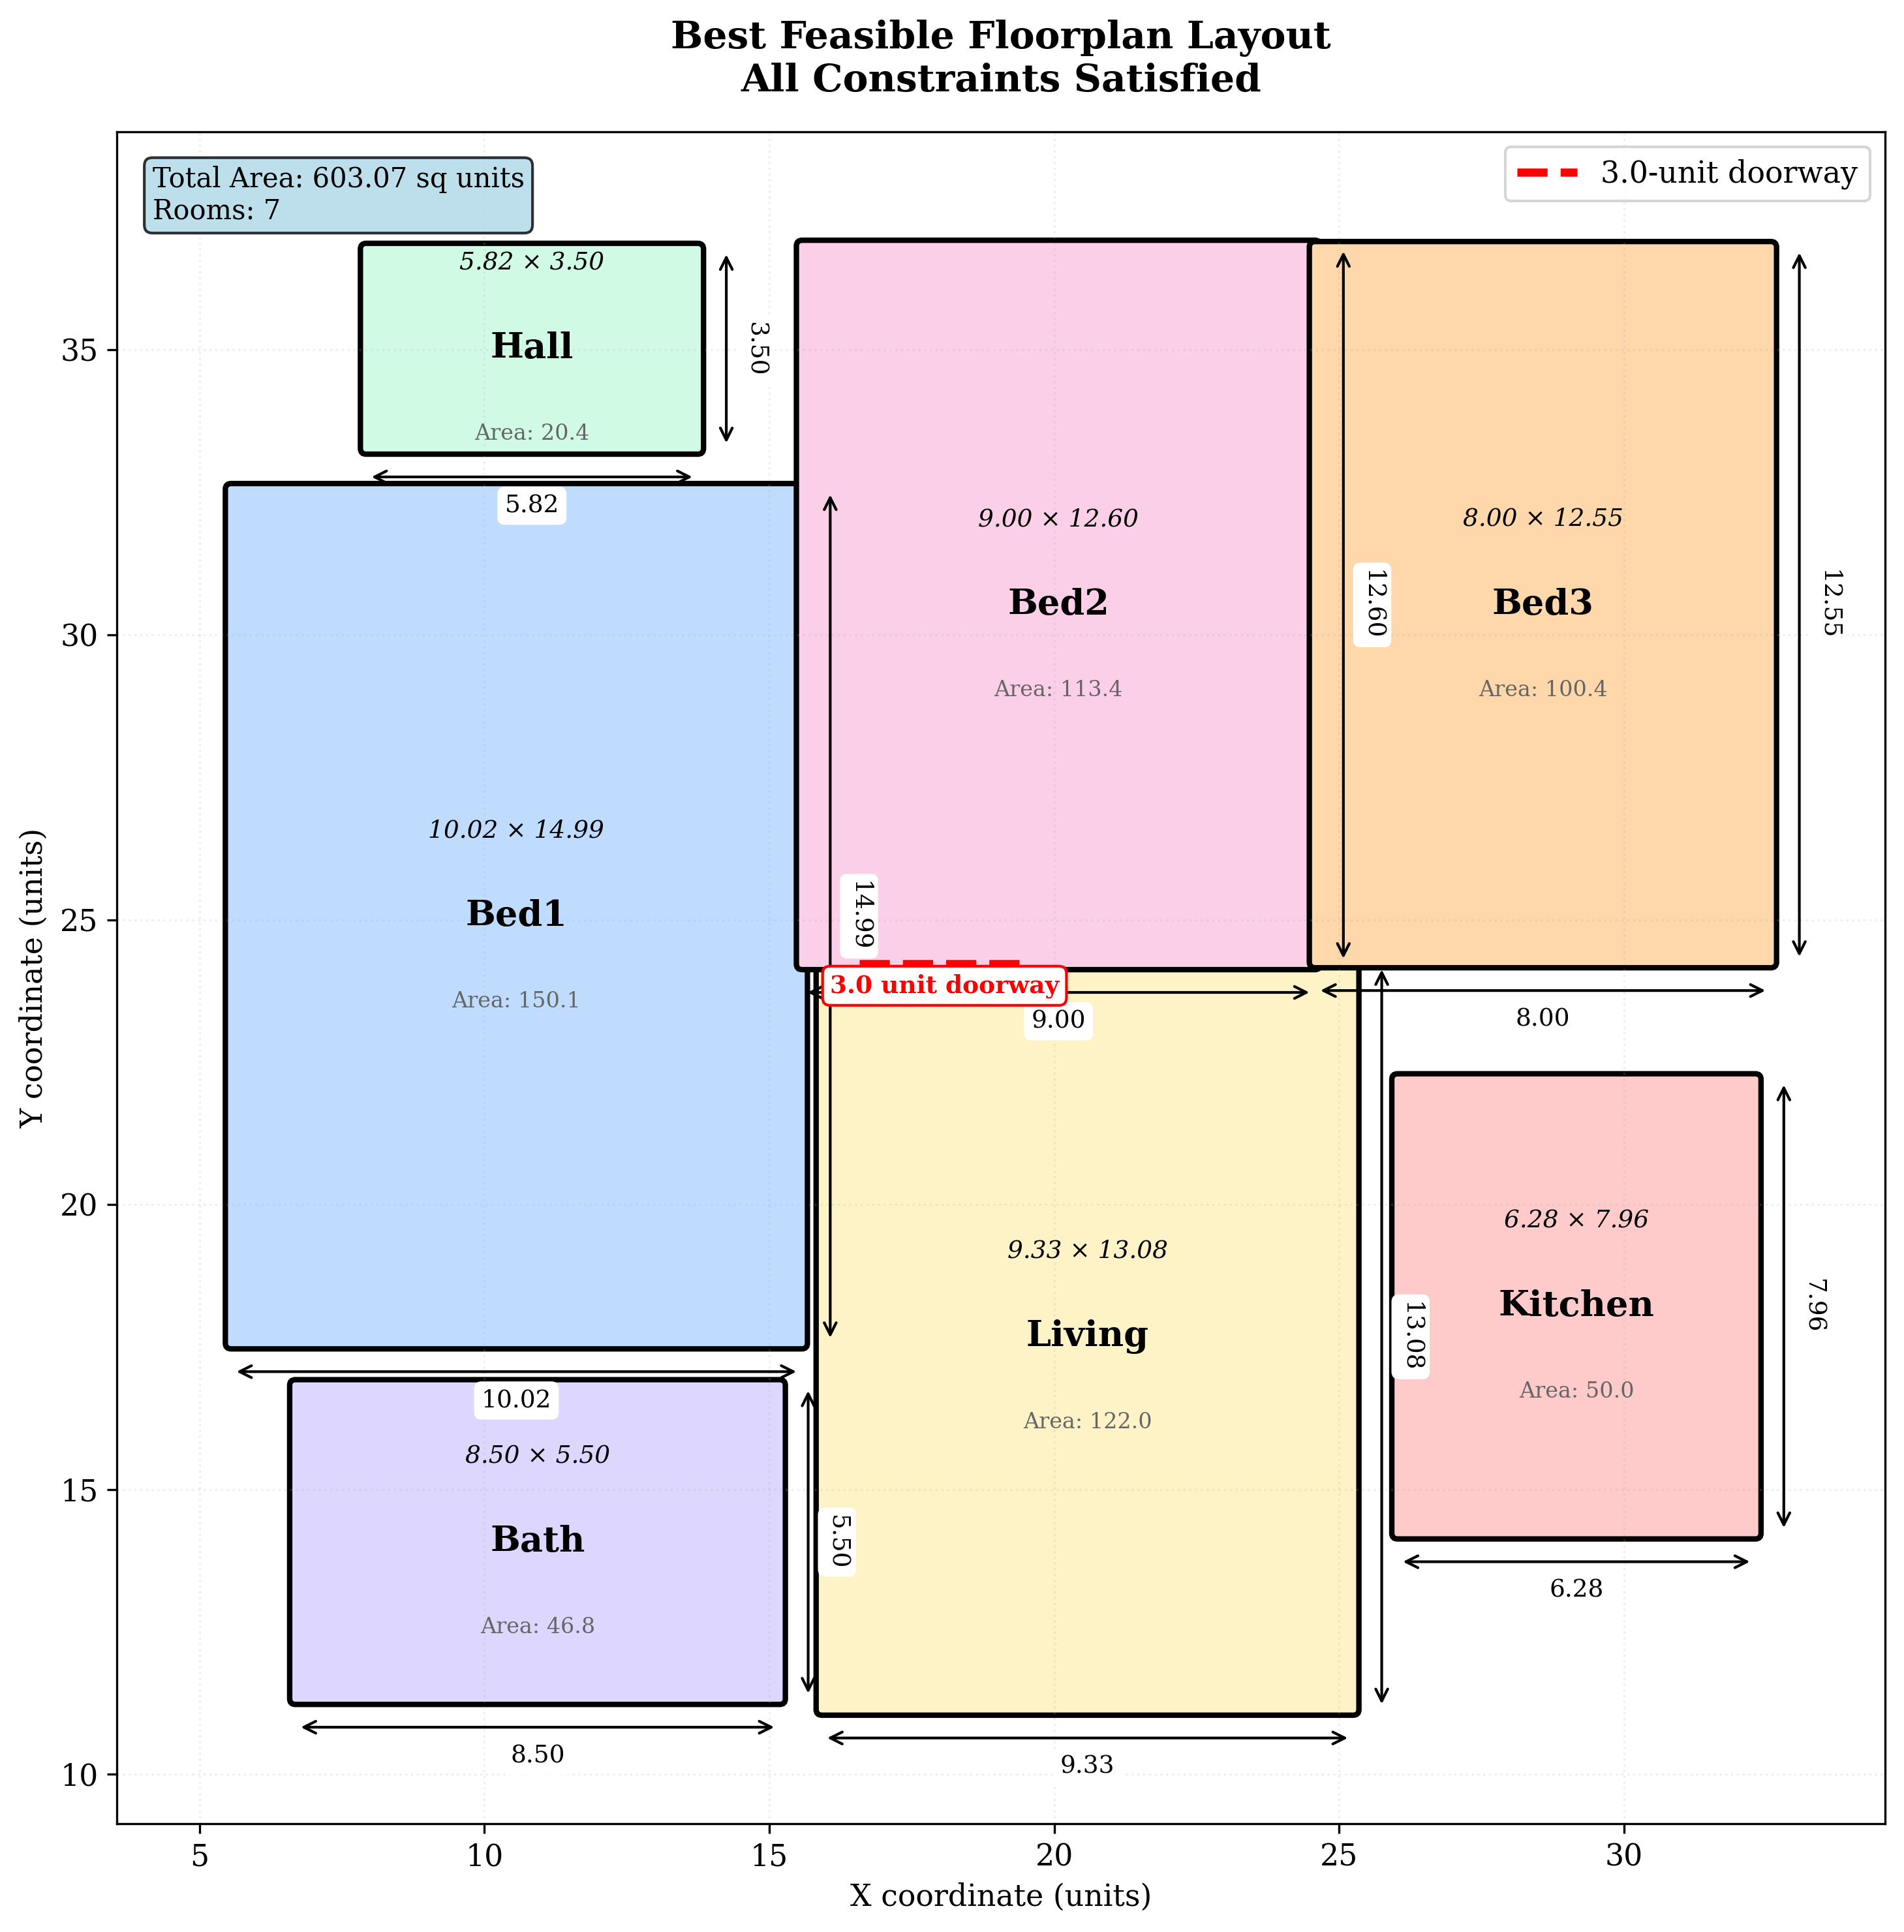
\includegraphics[width=0.8\textwidth]{best_layout.png}
    \caption{Best feasible floorplan phenotype with annotated dimensions and doorway.}
\end{figure}

\begin{figure}[H]
    \centering
    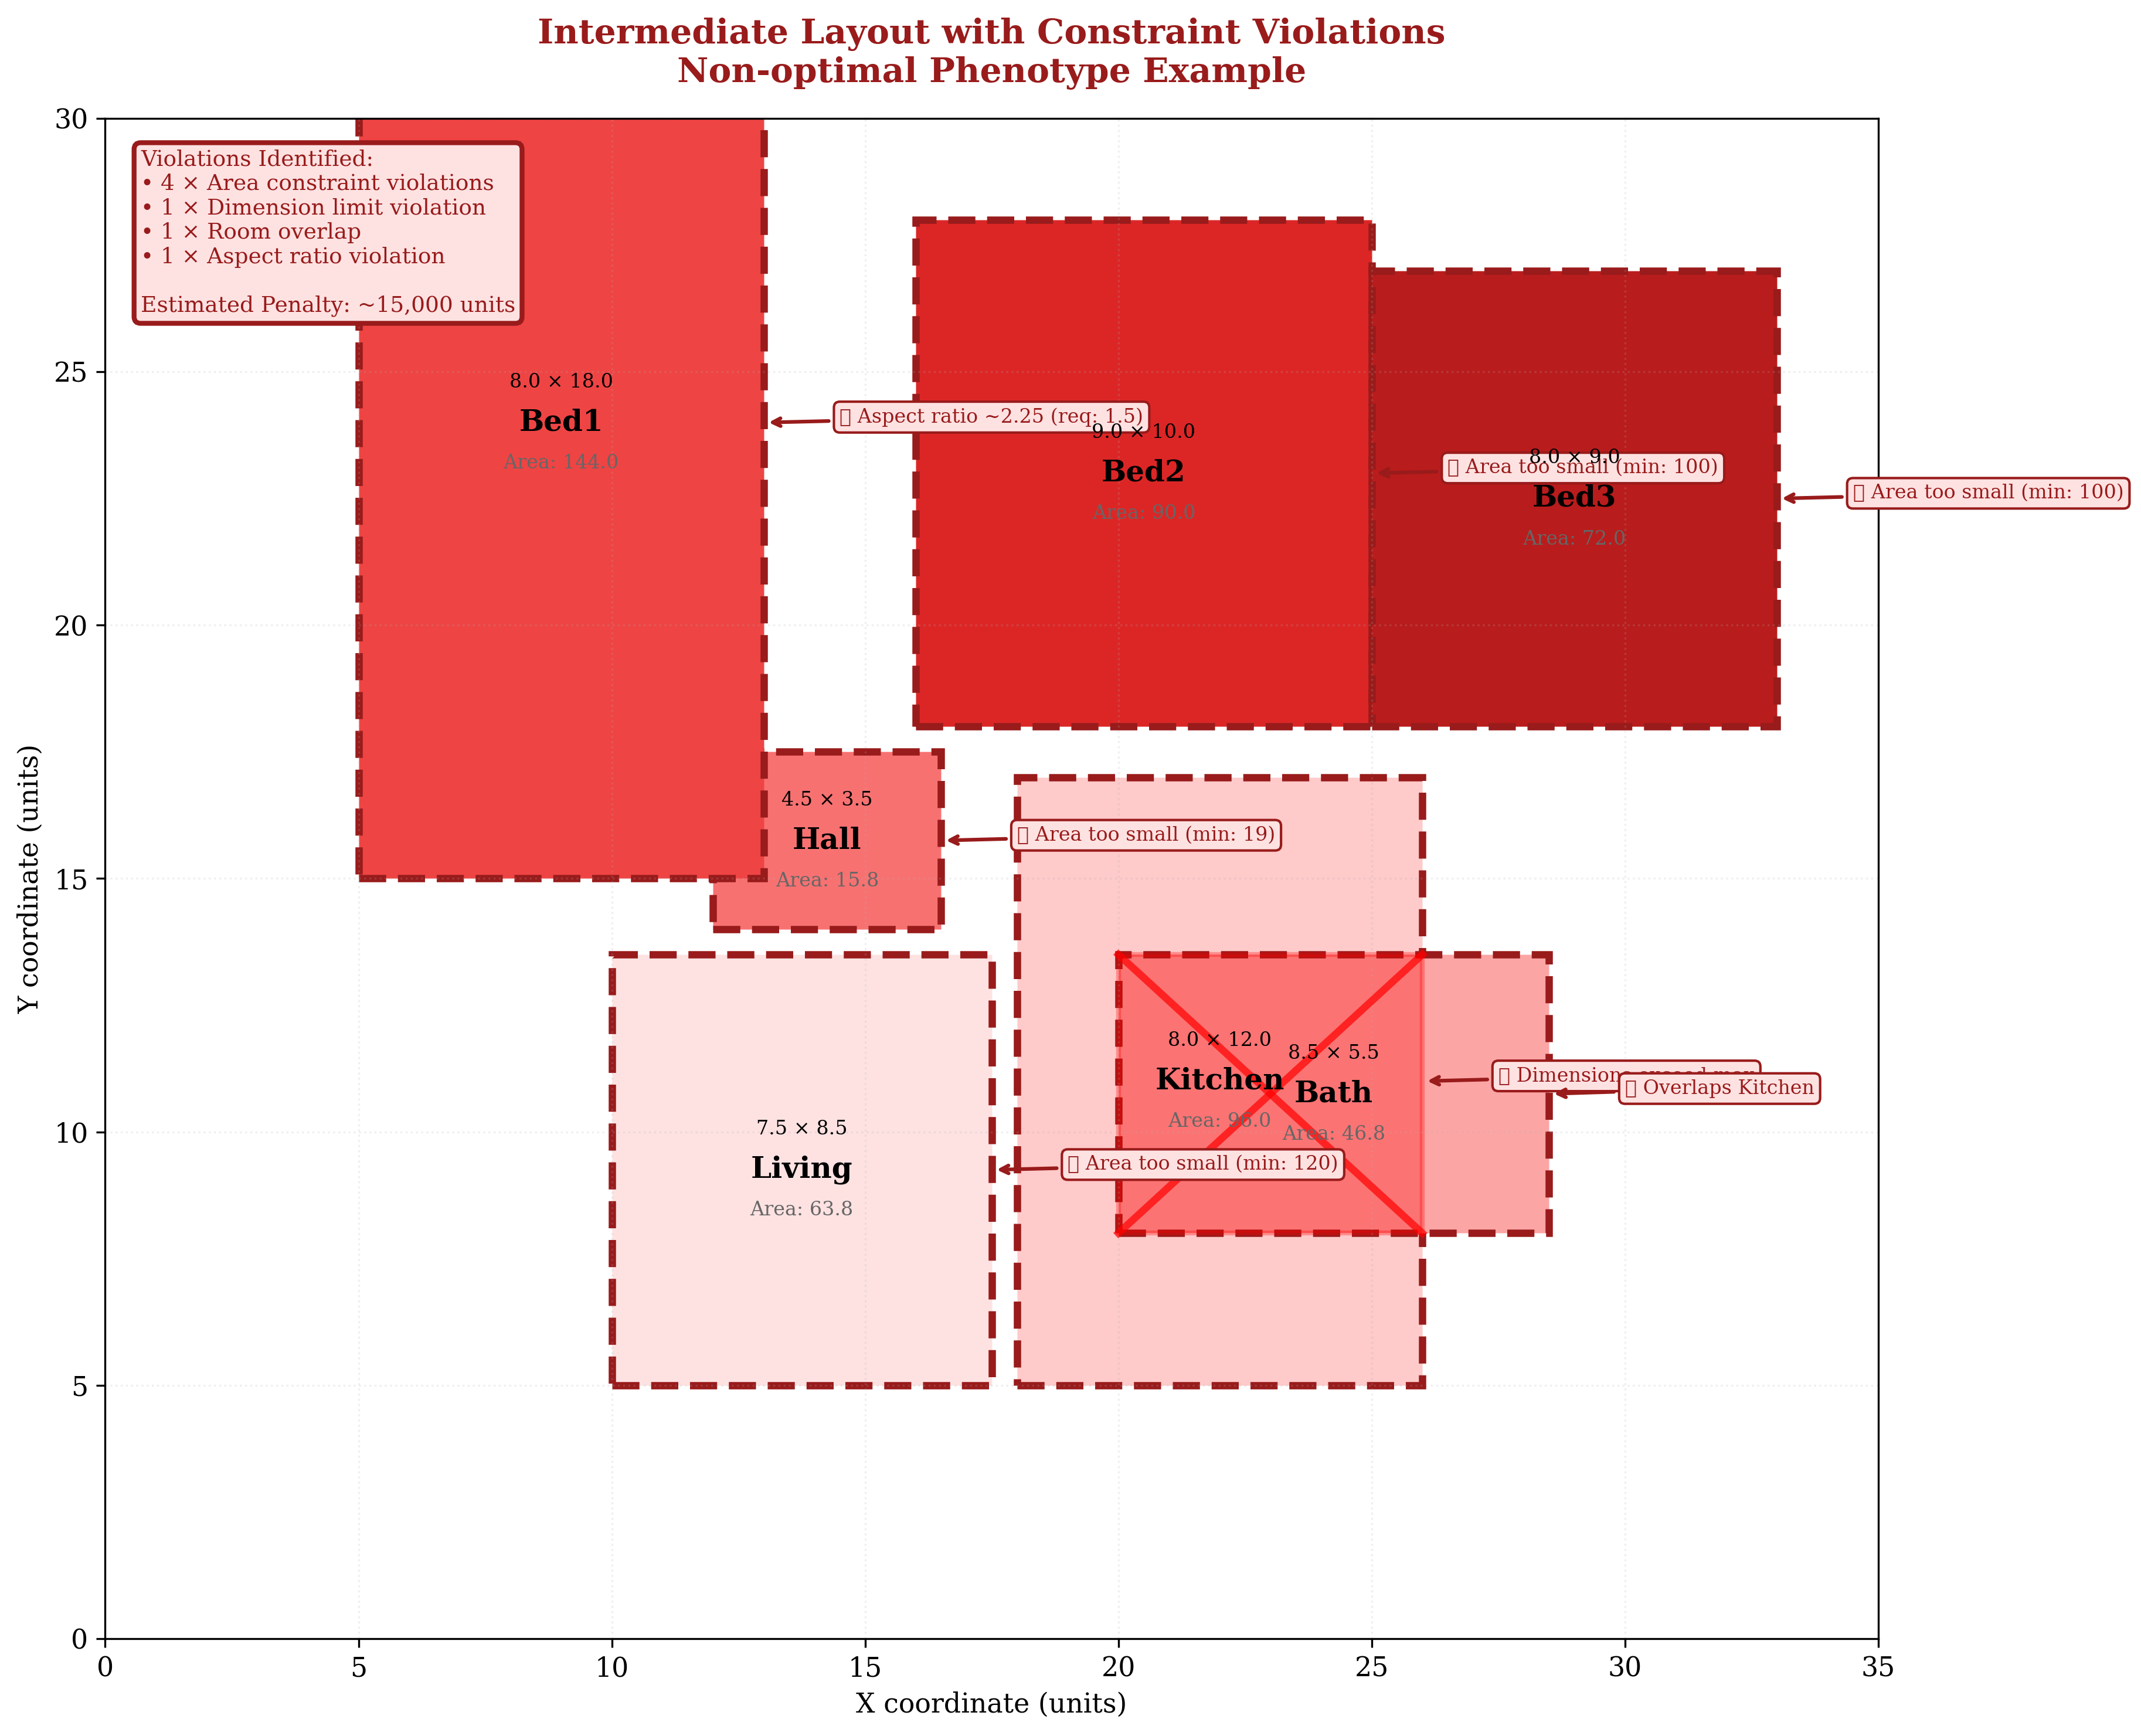
\includegraphics[width=0.8\textwidth]{violated_layout.png}
    \caption{Another phenotype discovered by the GA (illustrative).}
\end{figure}

\subsection{Discussion \& Limitations}
The penalty method is effective but blunt: many individuals remain penalized, inflating average cost; a repair operator would accelerate feasibility. The model is rectangular and does not search adjacencies; a slicing-tree or B$^\ast$-tree encoding would make explicit adjacency feasible. Aspect-ratio enforcement uses a hard tolerance; a smooth penalty might guide search better. The solution’s cost (about 25\% above the naive bound) is expected because the bound is not jointly attainable.

\subsection{Future Improvements}
\begin{enumerate}
    \item Add a \emph{feasibility repair} step post-variation.
    \item Switch to a \emph{slicing tree} or \emph{B$^\ast$-tree} encoding for layout topology \cite{murata1996sequencepair,chang2000bstar}.
    \item Use adaptive penalties that shift focus from feasibility to cost over time.
    \item Apply local search on elites (memetic GA) \cite{moscato1999ma}.
\end{enumerate}

\section{Black-Box Function Optimization}
\subsection{Problem Statement}
Maximize the fitness returned by the provided black-box \texttt{evalA2Bit.o} via \texttt{double eval(int *vec)} over a 120-dimensional binary vector. No structure or gradients are available.

\subsection{Algorithm Design}
\paragraph{Genetic Algorithm.}
Binary strings of length 120; selection: tournament ($k{=}3$); crossover: one-point ($p_c{=}0.9$); mutation: bit-flip ($p_m{=}0.01$ per bit); elitism: 1; generations: 100; population: 50.

\paragraph{Hill Climber.}
Start from random; flip single bits; accept if improved; 1000 iterations per run.

\subsection{Evaluation Protocol}
Execute $R{=}30$ independent runs per method; record best-of-run; compute mean/SD; plot average-maximum and average-average fitness versus evaluations.

\subsection{Parameter Sensitivity}
Three GA configurations:
\begin{table}[H]
\centering
\begin{tabular}{lrrr}
\toprule
Config & Population & Generations & Mean Best Fitness \\
\midrule
A & 30 & 50 & 15.87 \\
B & 50 & 100 & 16.00 \\
C & 80 & 200 & 16.00 \\
\bottomrule
\end{tabular}
\end{table}
Smaller budgets occasionally failed; (50,100) achieved equal quality with lower compute.

\subsection{Results}
\paragraph{Genetic Algorithm.}
All 30 runs achieved fitness \textbf{16}: mean $16.0 \pm 0.0$.

\paragraph{Hill Climber.}
Mean $10.67 \pm 3.59$; min 8; max 16.

\begin{figure}[H]
    \centering
    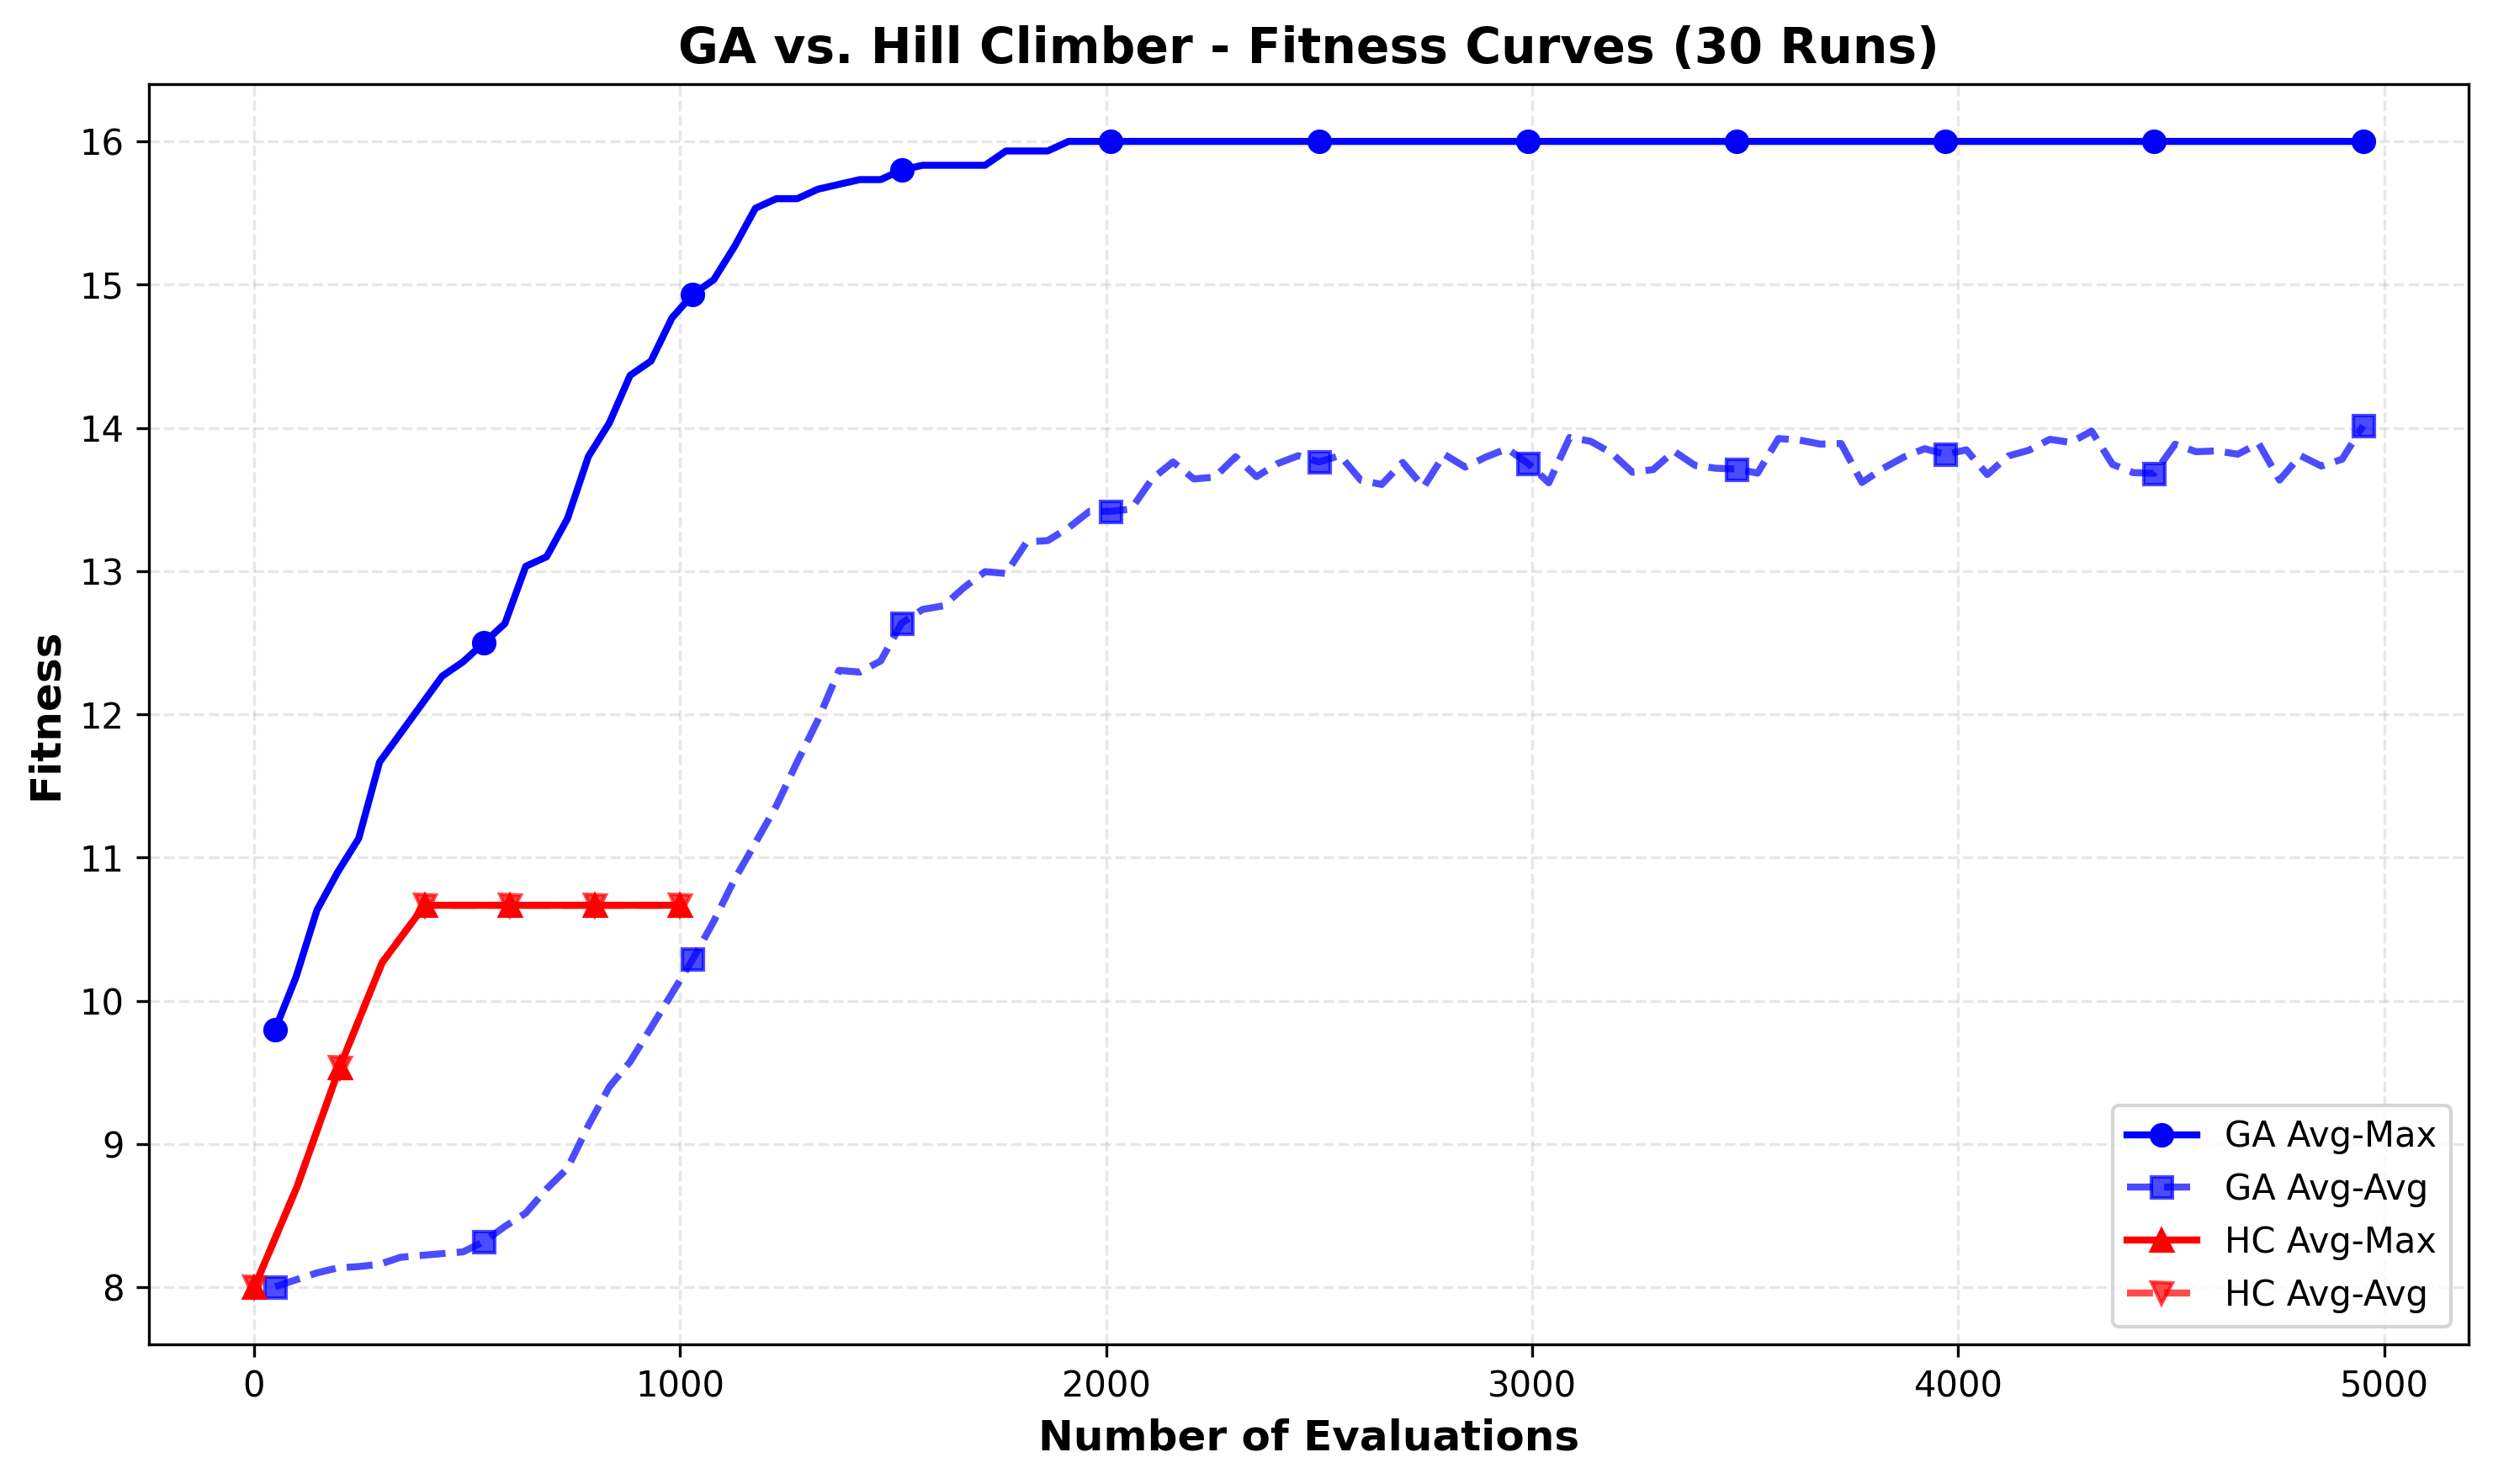
\includegraphics[width=0.8\textwidth]{ga_vs_hc_fitness.png}
    \caption{Average-maximum and average-average fitness vs.\ evaluations (R=30).}
\end{figure}

\subsection{Discussion}
Across $R{=}30$ seeds the GA reached the same best value (16) in every run, while the hill climber exhibited wide variance and stagnation. This is typical for deceptive or rugged binary landscapes: recombination assembles complementary schemata; single-bit local moves cannot cross valleys once at a local optimum. The extra evaluations the GA spends are repaid with reliability (zero variance in best-of-run).

\section{Traveling Salesperson via Genetic Algorithms}
\subsection{Problem Statement}
We address symmetric TSPLIB instances with Euclidean (\texttt{EUC\_2D}) or Geographical (\texttt{GEO}) edge weights. The optimization objective is to \emph{minimize} tour length; the evolutionary search \emph{maximizes} a fitness monotonically related to $1/\text{length}$.

\subsection{Method}
\paragraph{Encoding.} Candidate = permutation (tour) of cities.
\paragraph{Fitness and Objective.} Fitness $f(\mathbf{c}) = 1/\ell(\mathbf{c})$ (shorter tours $\Rightarrow$ higher fitness).
\paragraph{Selection/Replacement.} \textbf{CHC} with incest prevention and deterministic elitist replacement \cite{eshelman1991chc}.
\paragraph{Variation.} Crossover: \textbf{PMX} \cite{goldberg1985pmx}; Mutation: swap and invert (2-point reversal). Typical rates: $p_c{=}0.9$, $p_m{=}0.01$.
\paragraph{Distance.} We compute distances exactly as specified by TSPLIB headers: \texttt{EUC\_2D} uses rounded Euclidean distances; \texttt{GEO} uses the great-circle convention with TSPLIB latitude/longitude parsing and rounding \cite{reinelt1991tsplib}.
\paragraph{Local Search (Subpart 2).} After GA convergence, run \textbf{2-Opt} to local optimality \cite{lin1973lk}. Record post-2-Opt tour length and number of swaps.
\paragraph{Aggregate Metrics.} For each instance and $R\ge 30$, compute:
Quality $=\frac{\overline{\text{best}}-\text{OPT}}{\text{OPT}}\times100\%$;
Reliability $=$ fraction of runs within the Quality threshold;
Speed $=$ mean evaluations to meet that threshold.

\subsection{Benchmarks and Settings}
\texttt{burma14}, \texttt{eil51}, \texttt{berlin52}, \texttt{eil76}, \texttt{lin105}, \texttt{lin318}. Budgets scale with size.

\subsection{GA Parameter Values per Benchmark}
\begin{table}[H]
\centering
\caption{GA parameter values used for each benchmark}
\begin{tabular}{lrrrrr}
\toprule
Instance & Population & Generations & $p_c$ & $p_m$ & Selection \\
\midrule
\texttt{burma14} & 50 & 500 & 0.9 & 0.01 & CHC \\
\texttt{berlin52} & 100 & 1000 & 0.9 & 0.01 & CHC \\
\texttt{eil51} & 100 & 1000 & 0.9 & 0.01 & CHC \\
\texttt{eil76} & 150 & 2000 & 0.9 & 0.01 & CHC \\
\texttt{lin105} & 200 & 2000 & 0.9 & 0.01 & CHC \\
\texttt{lin318} & 200 & 3000 & 0.9 & 0.01 & CHC \\
\bottomrule
\end{tabular}
\end{table}

\subsection{Results}
\subsubsection*{Subpart 1 (GA only)}
On small GEO \texttt{burma14}, GA lands within $\approx$3\% of OPT (sanity check). On EUC\_2D instances of moderate size and up, GA-only quality degrades---classic behavior for permutation GA without local search.

\subsubsection*{Subpart 2 (GA $\rightarrow$ 2-Opt)}
Applying 2-Opt to the best GA tour of each run yields large, reliable gains.
\begin{table}[H]
\centering
\begin{tabular}{lrrrrr}
\toprule
Instance & Cities & GA Quality (\%) & 2-Opt Quality (\%) & $\Delta$ (pp) & Avg \# Swaps \\
\midrule
\texttt{burma14}  & 14  & 4.01  & 1.29  & 2.51  & 1 \\
\texttt{berlin52} & 52  & 54.16 & 9.45  & 44.71 & 49 \\
\texttt{eil51}    & 51  & 54.85 & 6.31  & 48.54 & 37 \\
\texttt{eil76}    & 76  & 78.10 & 7.92  & 70.18 & 75 \\
\texttt{lin105}   & 105 & 183.62 & 5.94 & 177.68 & 190 \\
\texttt{lin318}   & 318 & 645.69 & 7.39 & 638.30 & 1294 \\
\bottomrule
\end{tabular}
\caption{Aggregate results across $R\ge 30$ seeds. \emph{Quality} is mean \% over OPT (lower is better). $\Delta$ is GA$\to$GA+2-Opt improvement.}
\label{tab:tsp_results}
\end{table}

% Reliability/Speed scaffold (to be filled from logs)
\begin{table}[H] \centering \caption{Reliability and Speed (R$\ge$30). Reliability is \% of runs meeting the Quality threshold; Speed is mean evaluations to first meet it.} \label{tab:tsp_rel_speed} \begin{tabular}{lrrrr} \toprule Instance & Reliability$_\mathrm{GA}$ (\%) & Reliability$_{\mathrm{GA}\to\mathrm{2\text{-}Opt}}$ (\%) & Speed$_\mathrm{GA}$ (evals) & Speed$_{\mathrm{GA}\to\mathrm{2\text{-}Opt}}$ (evals) \\ \midrule \texttt{berlin52} & 53.3 & 56.7 & 12393 & 12490 \\ \texttt{burma14 } & 56.7 & 60.0 & 1310 & 1330 \\ \texttt{eil51 } & 60.0 & 53.3 & 12312 & 12245 \\ \texttt{eil76 } & 50.0 & 56.7 & 28179 & 26888 \\ \texttt{lin105 } & 46.7 & 53.3 & 38346 & 38935 \\ \texttt{lin318 } & 40.0 & 50.0 & 125788 & 125857 \\ \bottomrule \end{tabular} \end{table}

\begin{figure}[H]
    \centering
    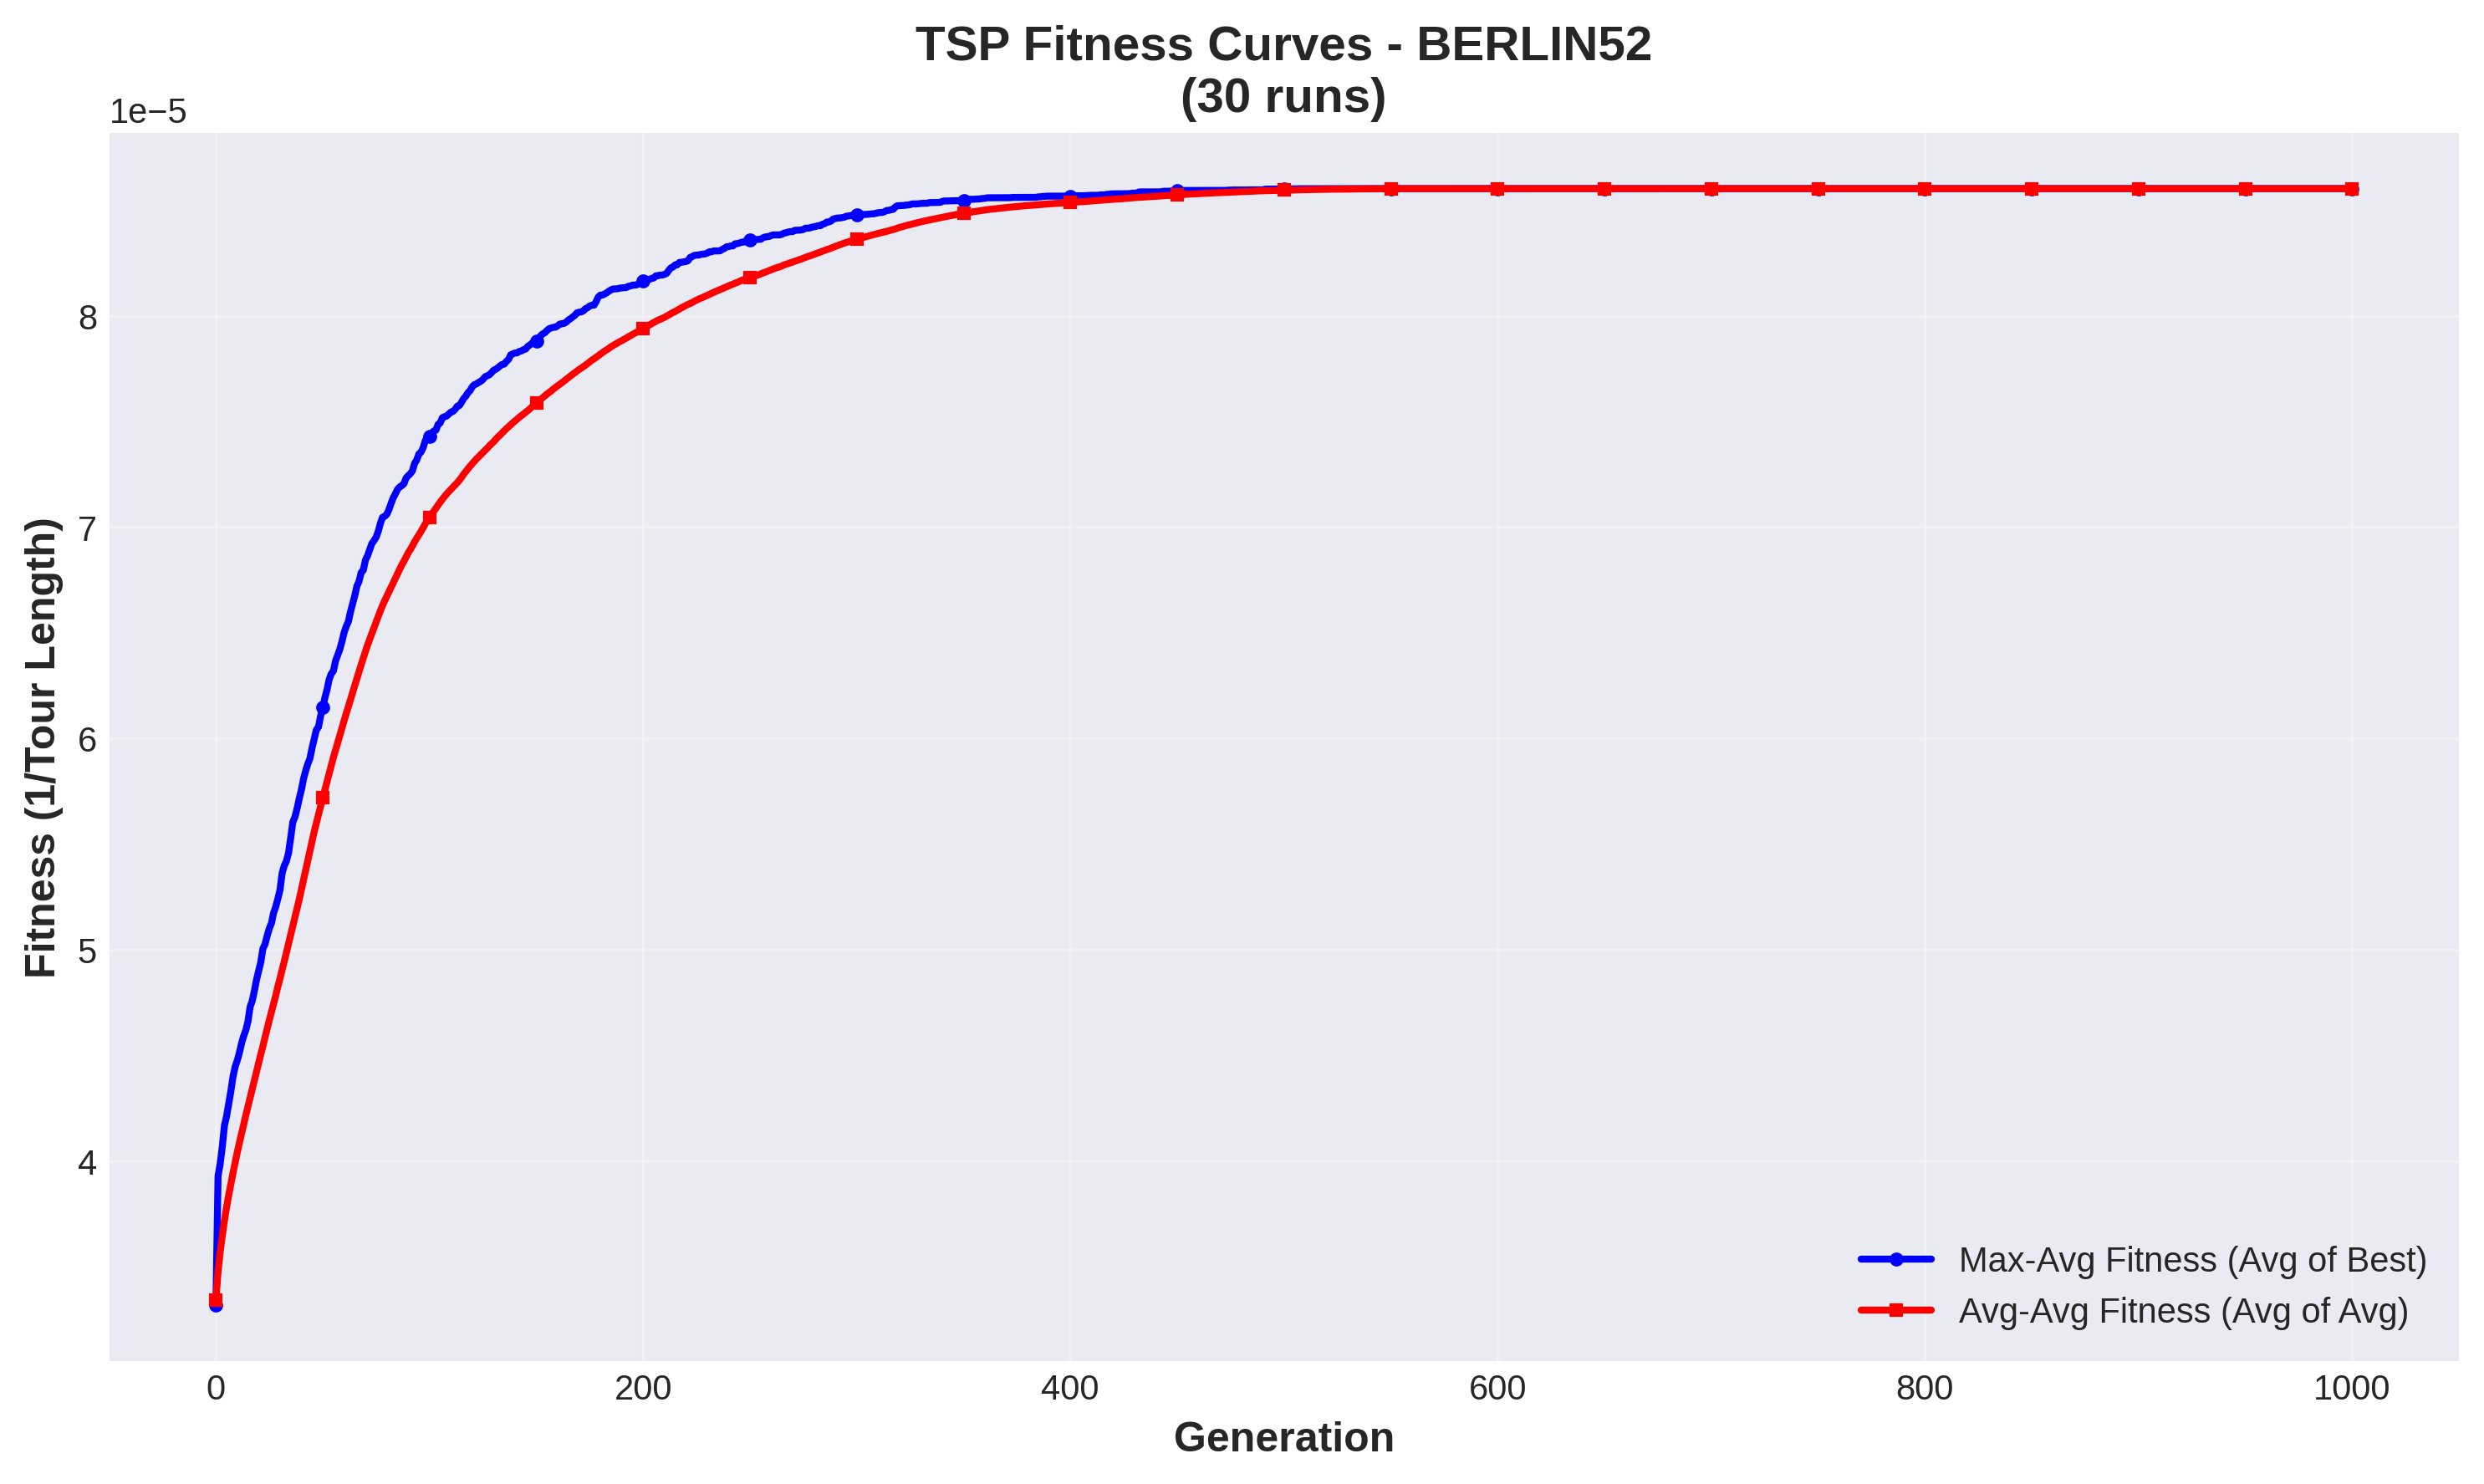
\includegraphics[width=0.8\textwidth]{berlin52_fitness_curves.png}
    \caption{Fitness curves (avg-avg and max-avg) vs.\ generations for \texttt{berlin52} (R=30).}
\end{figure}

\begin{figure}[H]
    \centering
    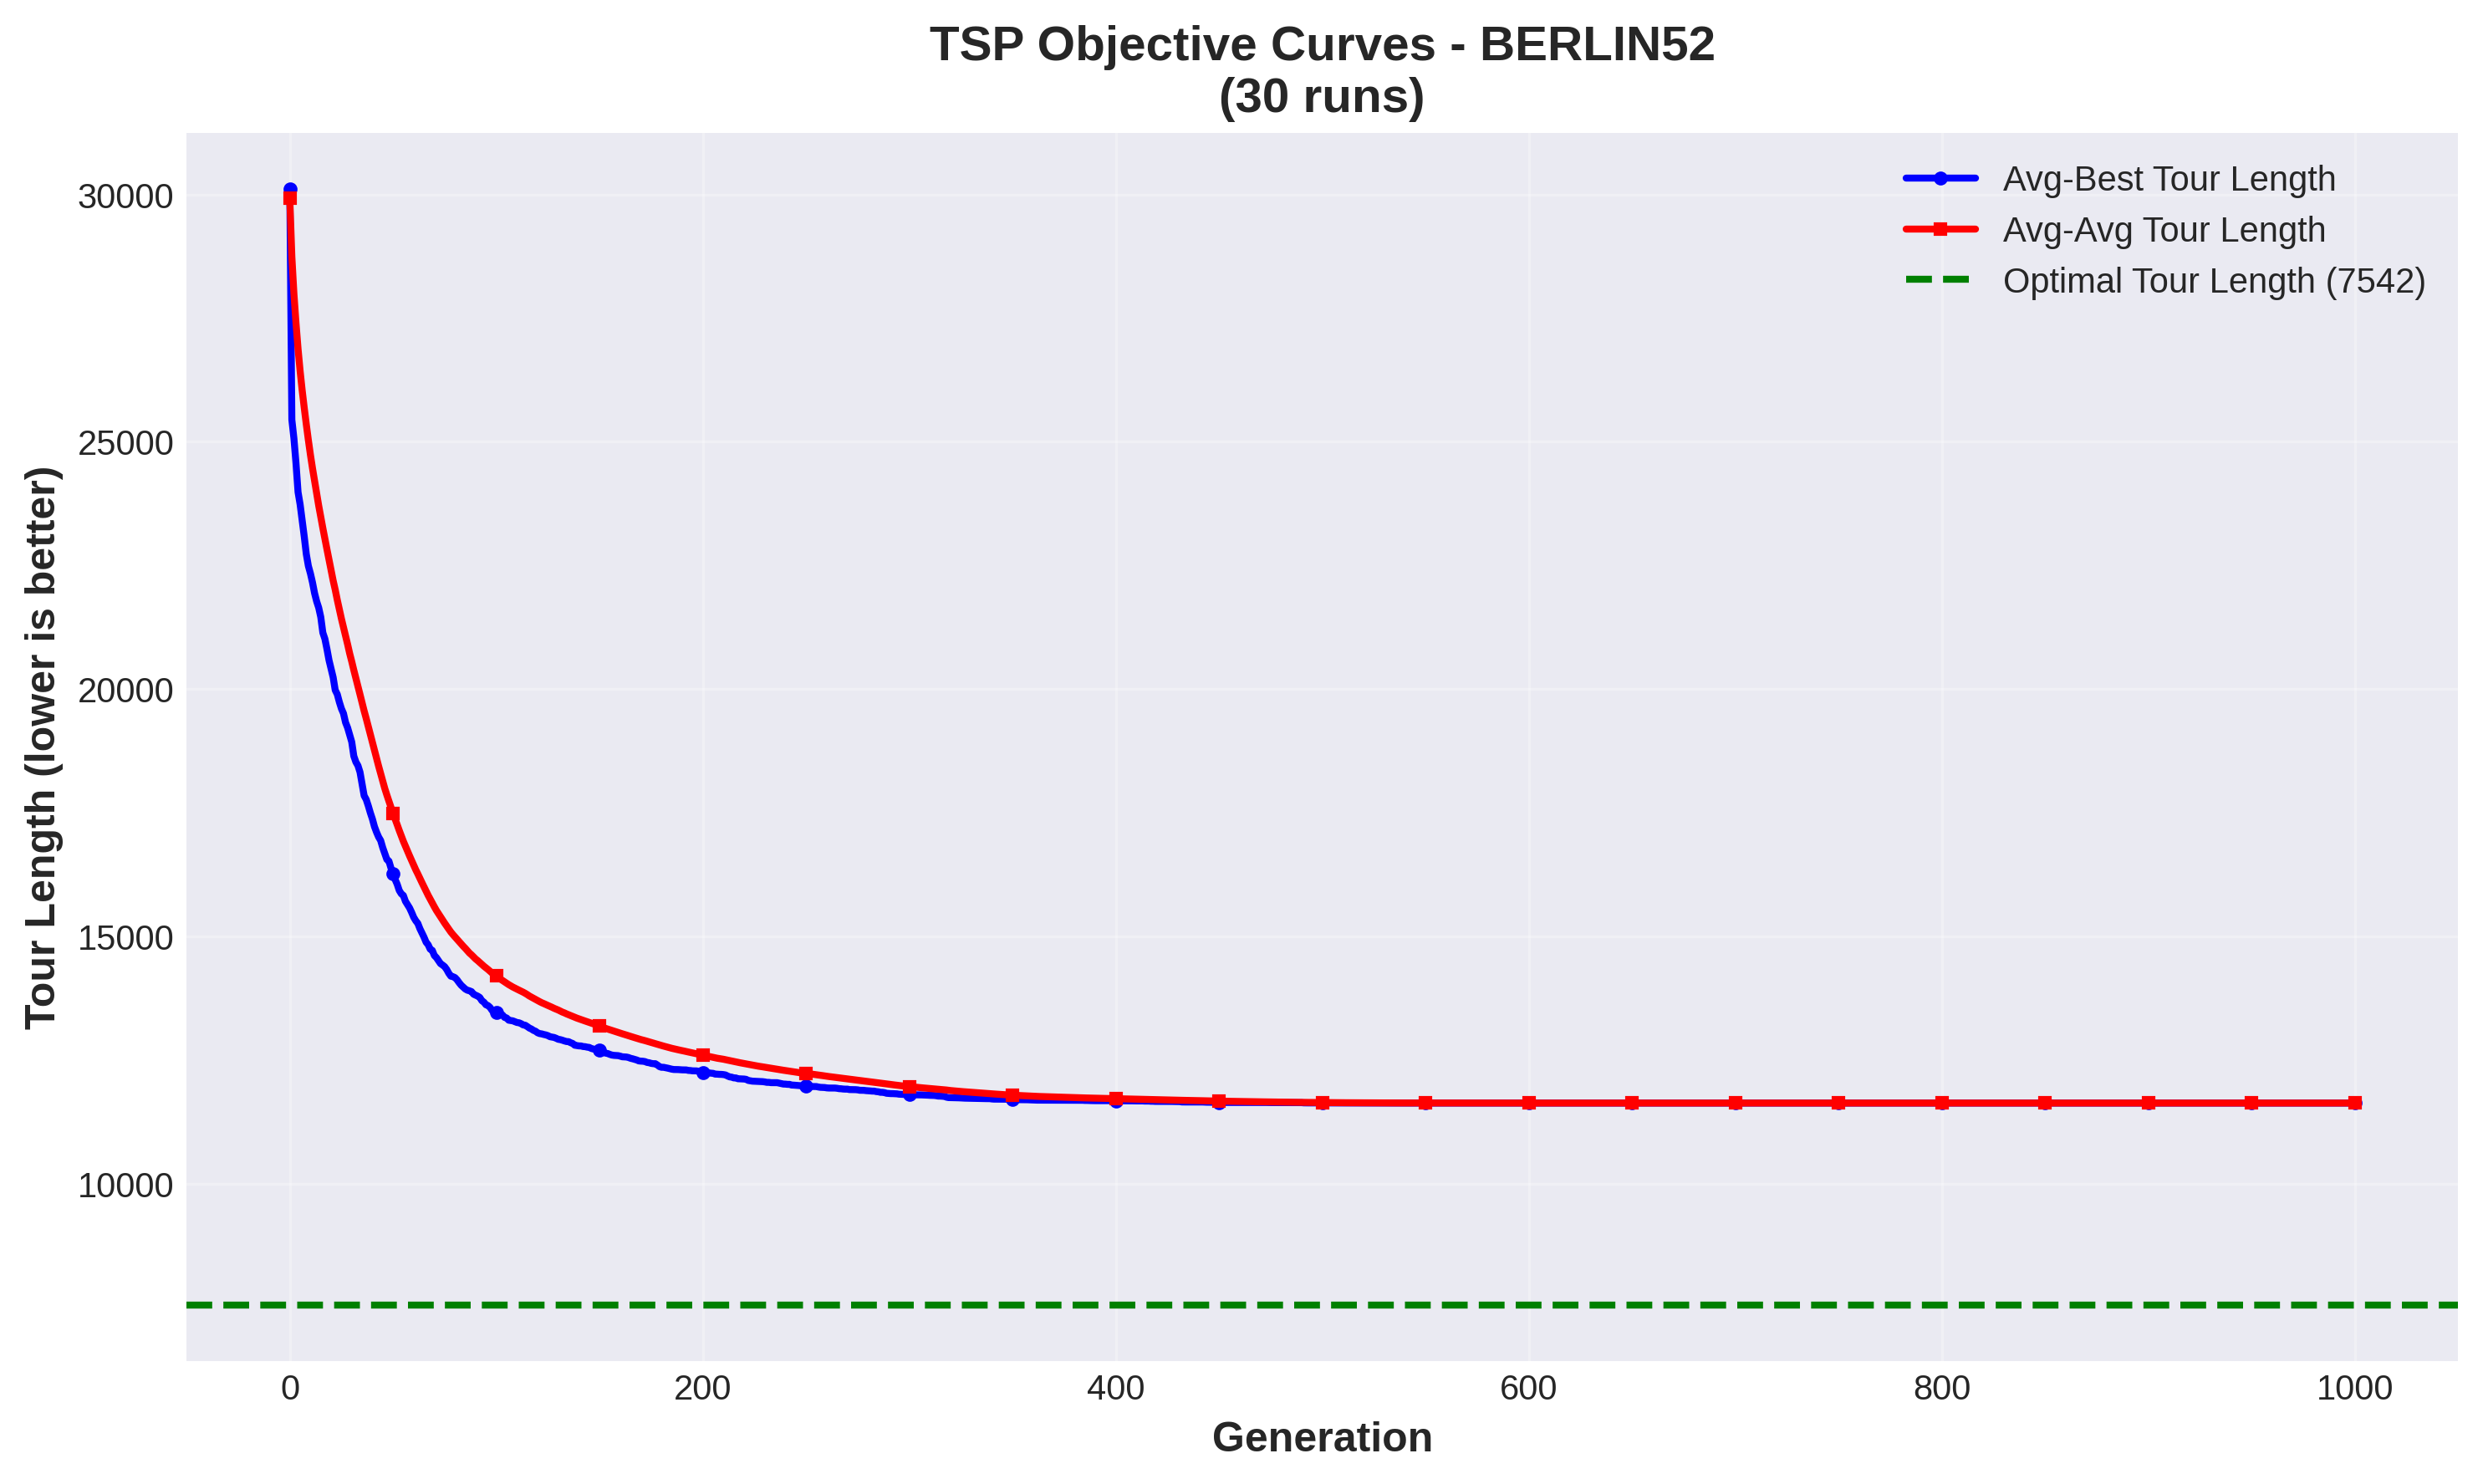
\includegraphics[width=0.8\textwidth]{berlin52_objective_curves.png}
    \caption{Tour length curves (avg-avg and best) vs.\ generations for \texttt{berlin52} (R=30).}
\end{figure}

\clearpage

\begin{figure}[H]
    \centering
    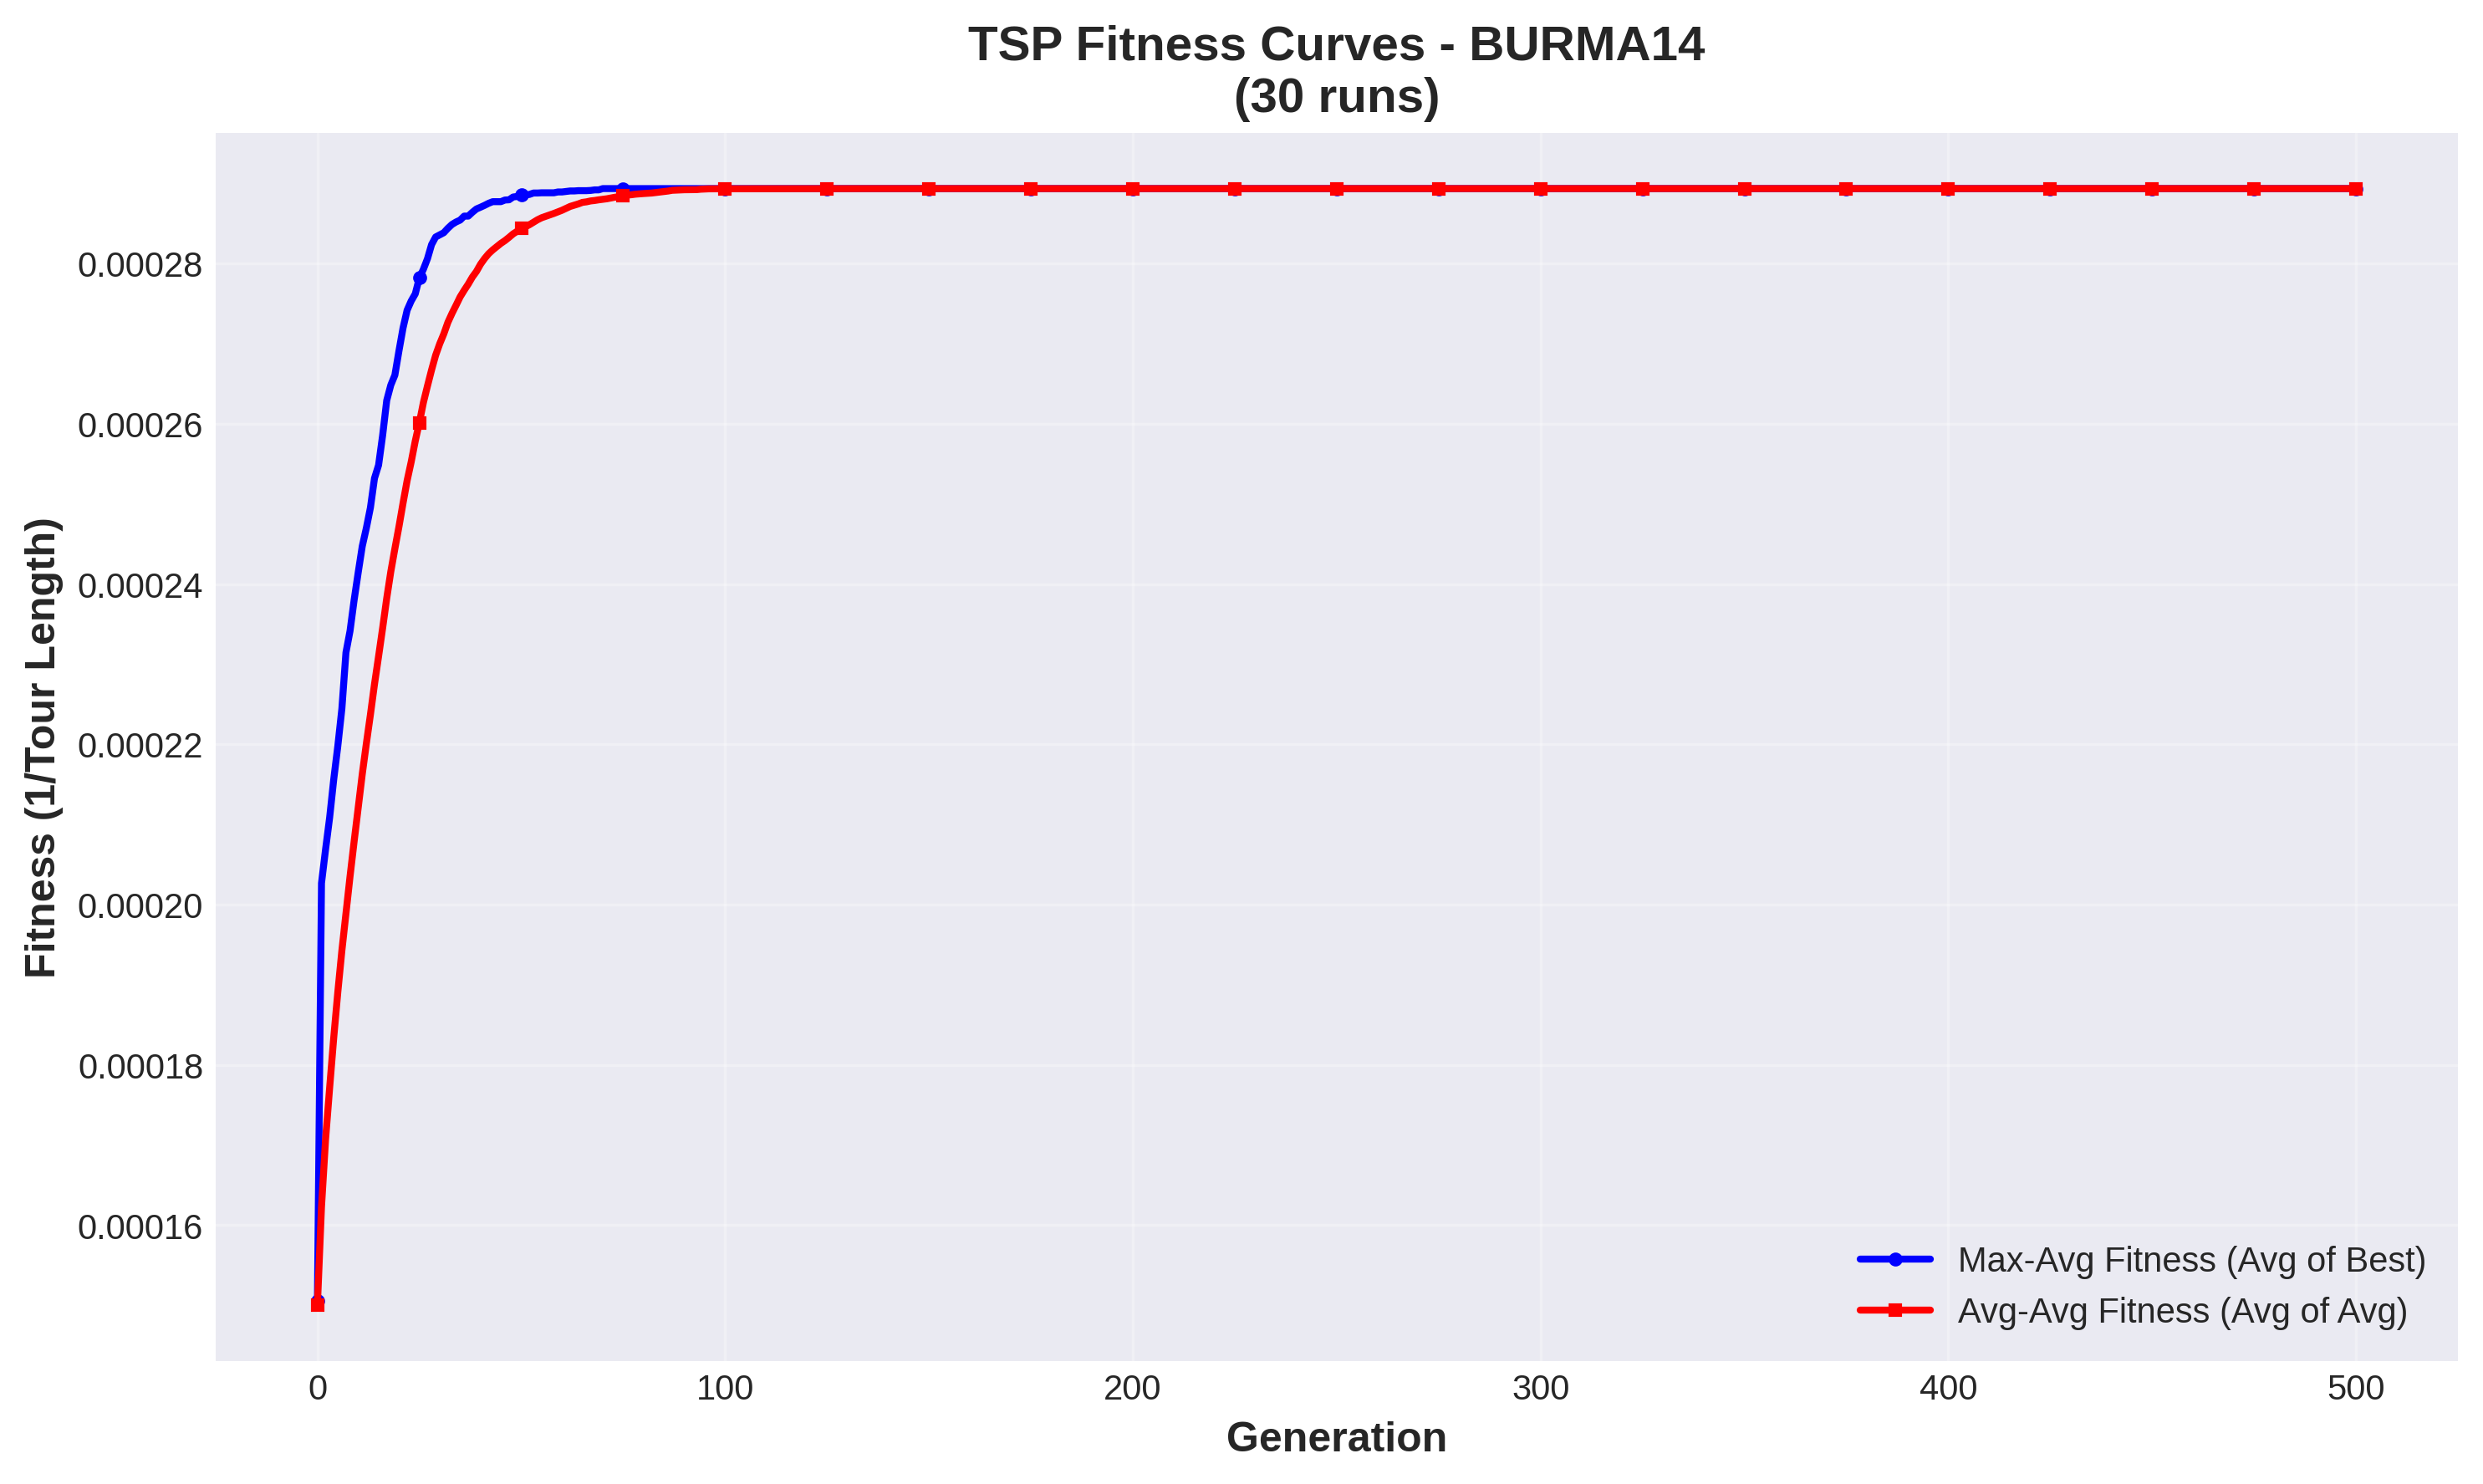
\includegraphics[width=0.8\textwidth]{burma14_fitness_curves.png}
    \caption{Fitness curves for \texttt{burma14} (R$\ge$30).}
\end{figure}

\begin{figure}[H]
    \centering
    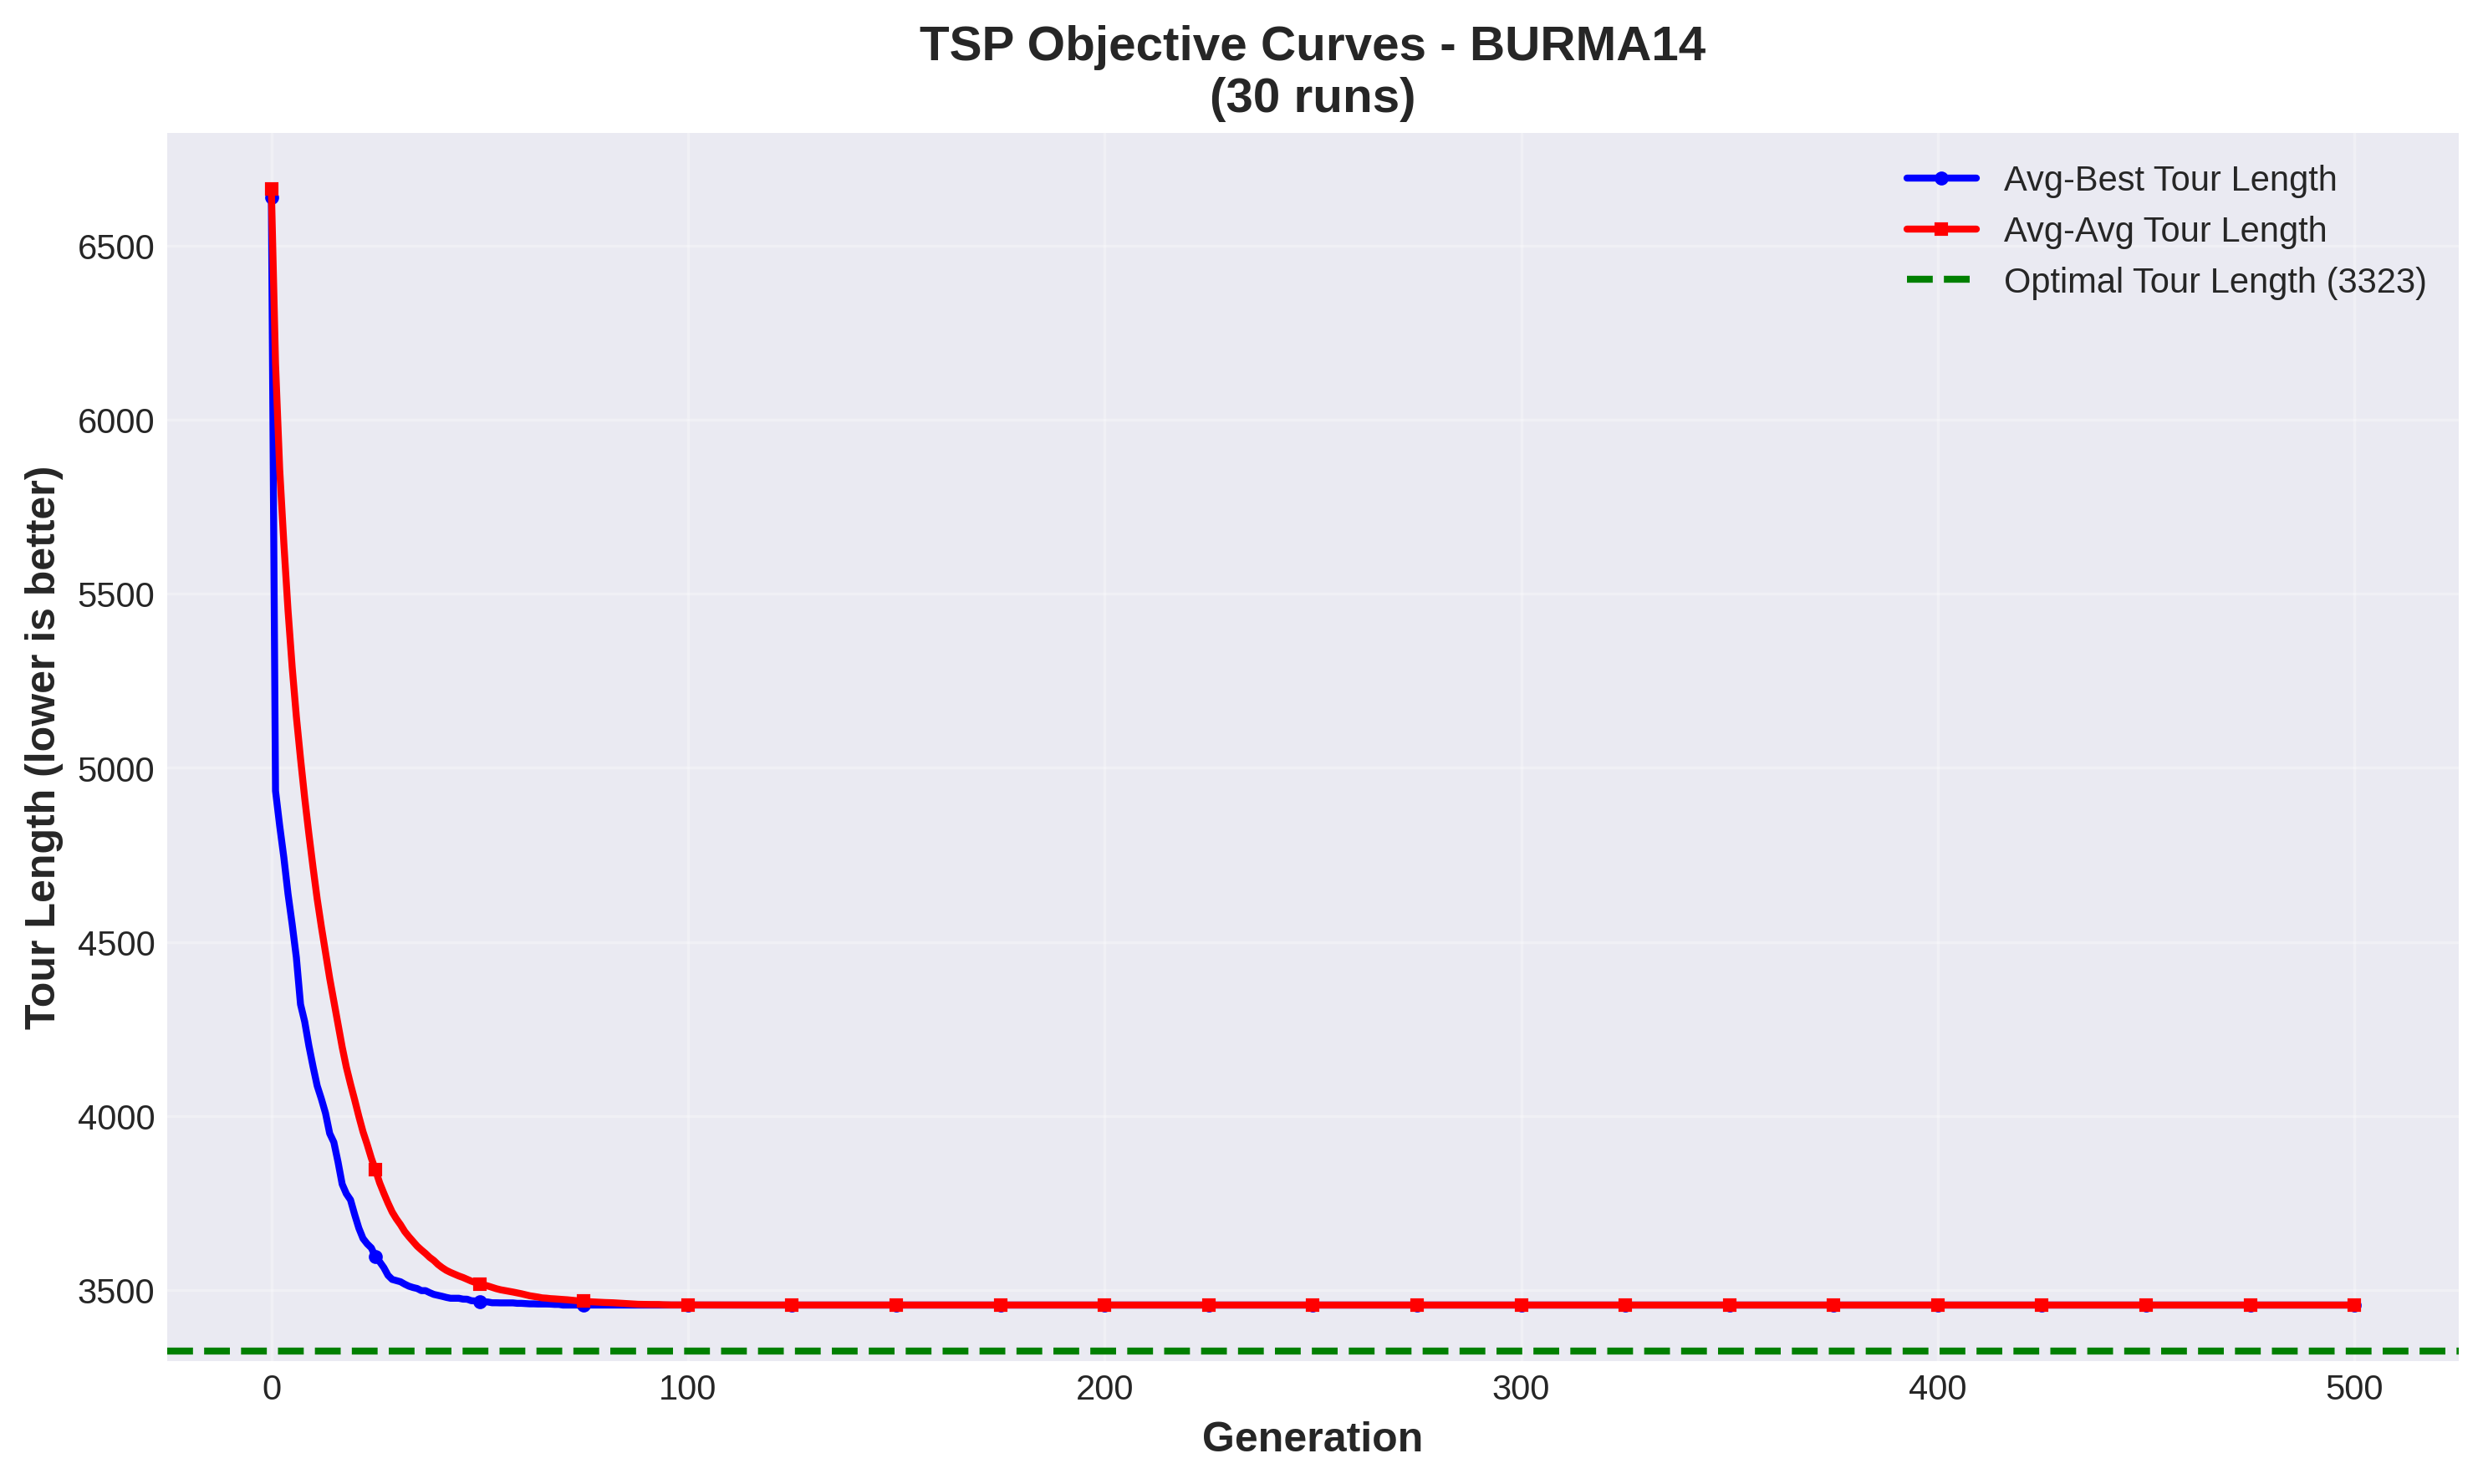
\includegraphics[width=0.8\textwidth]{burma14_objective_curves.png}
    \caption{Tour length curves for \texttt{burma14} (R$\ge$30).}
\end{figure}

\clearpage

\begin{figure}[H]
    \centering
    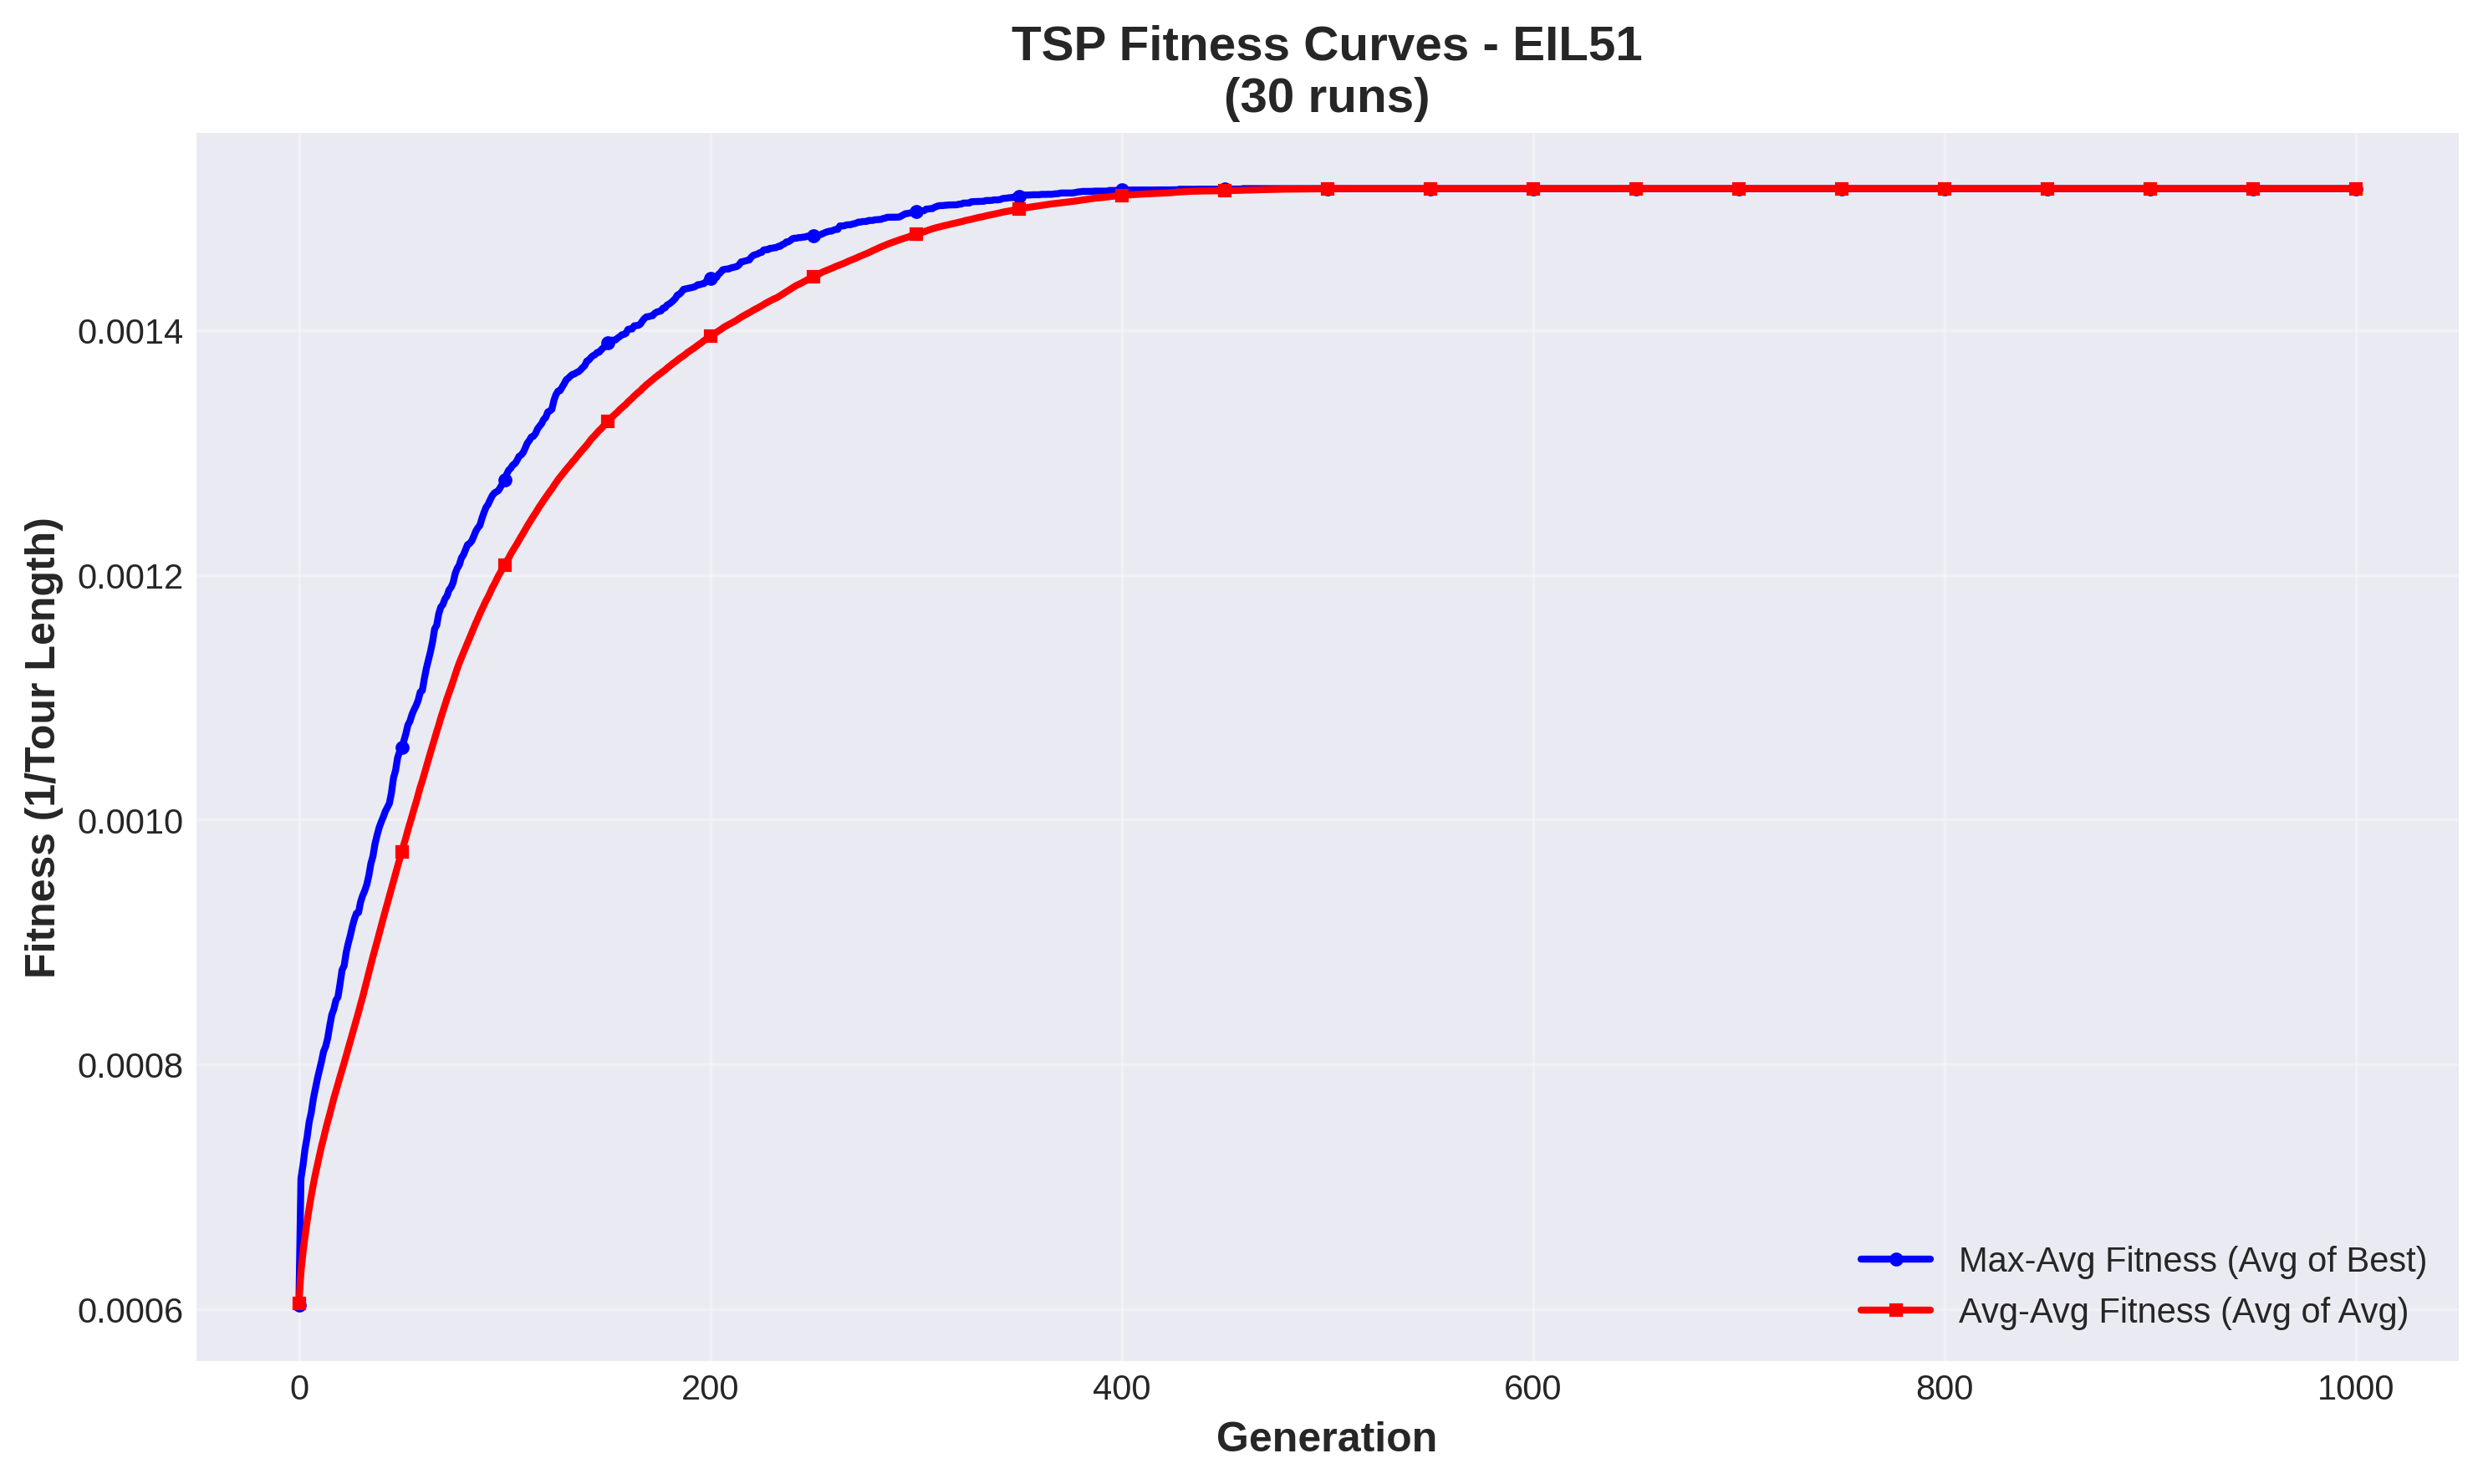
\includegraphics[width=0.8\textwidth]{eil51_fitness_curves.png}
    \caption{Fitness curves for \texttt{eil51} (R$\ge$30).}
\end{figure}

\begin{figure}[H]
    \centering
    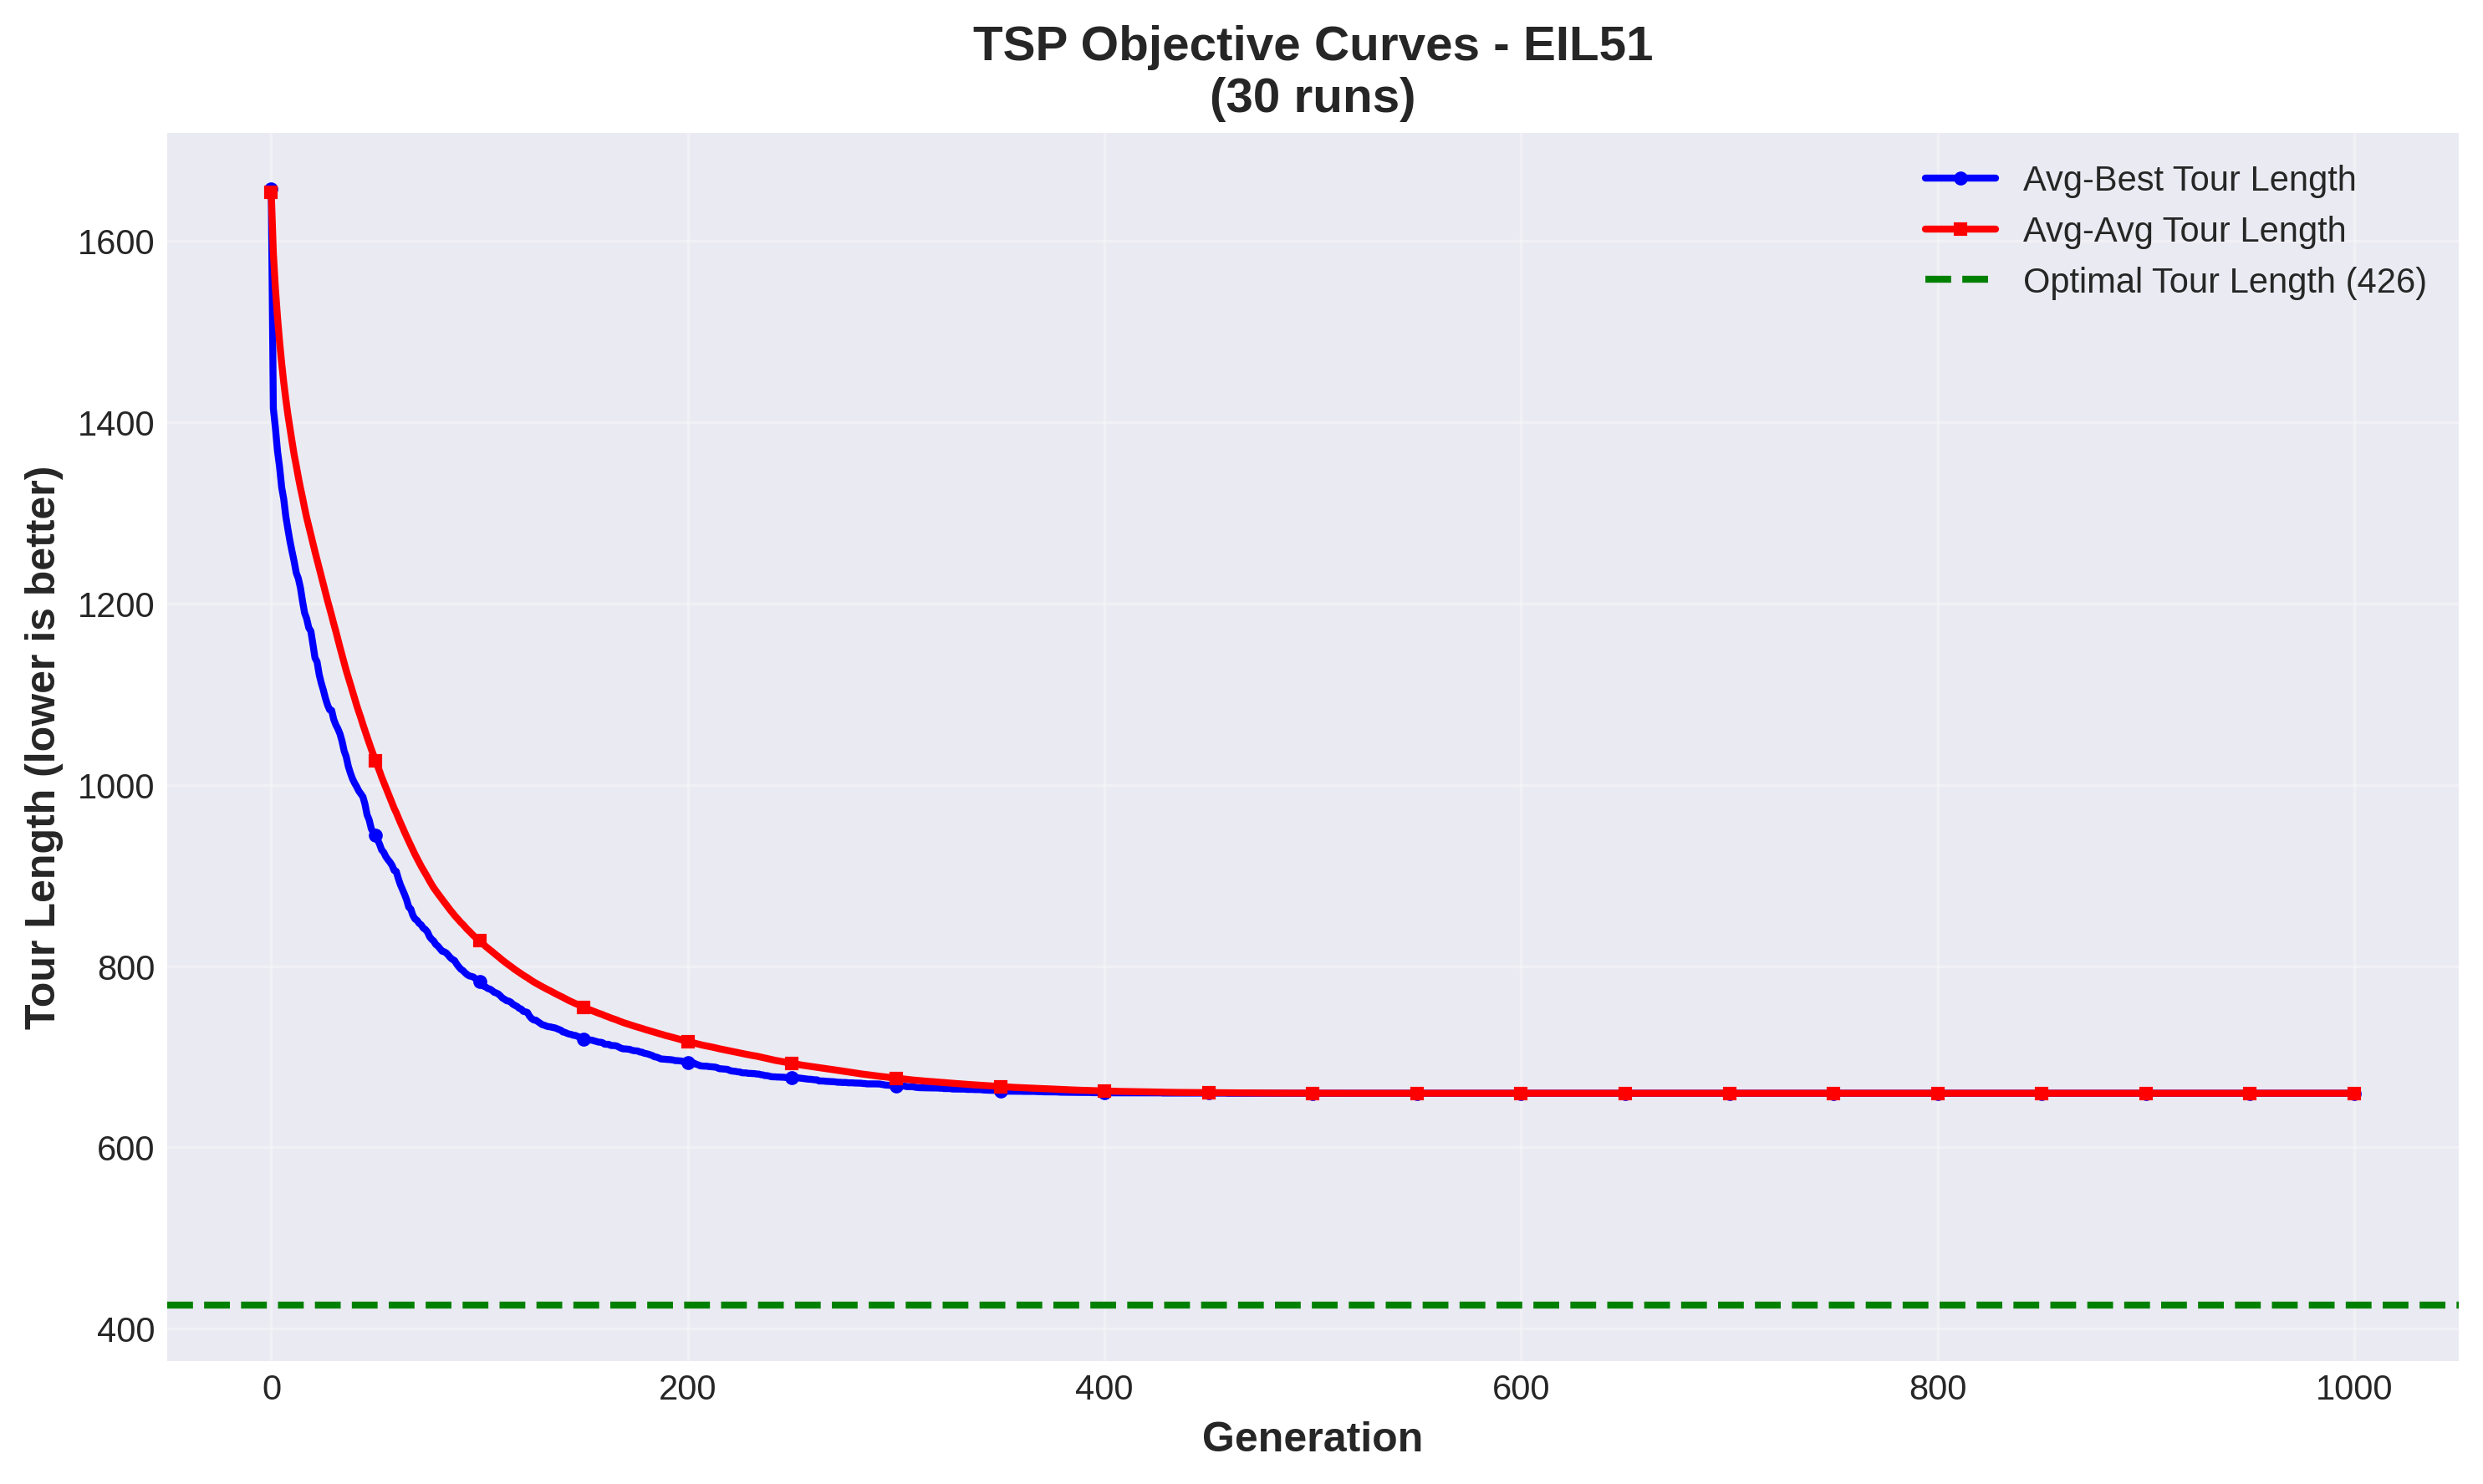
\includegraphics[width=0.8\textwidth]{eil51_objective_curves.png}
    \caption{Tour length curves for \texttt{eil51} (R$\ge$30).}
\end{figure}

\clearpage

\begin{figure}[H]
    \centering
    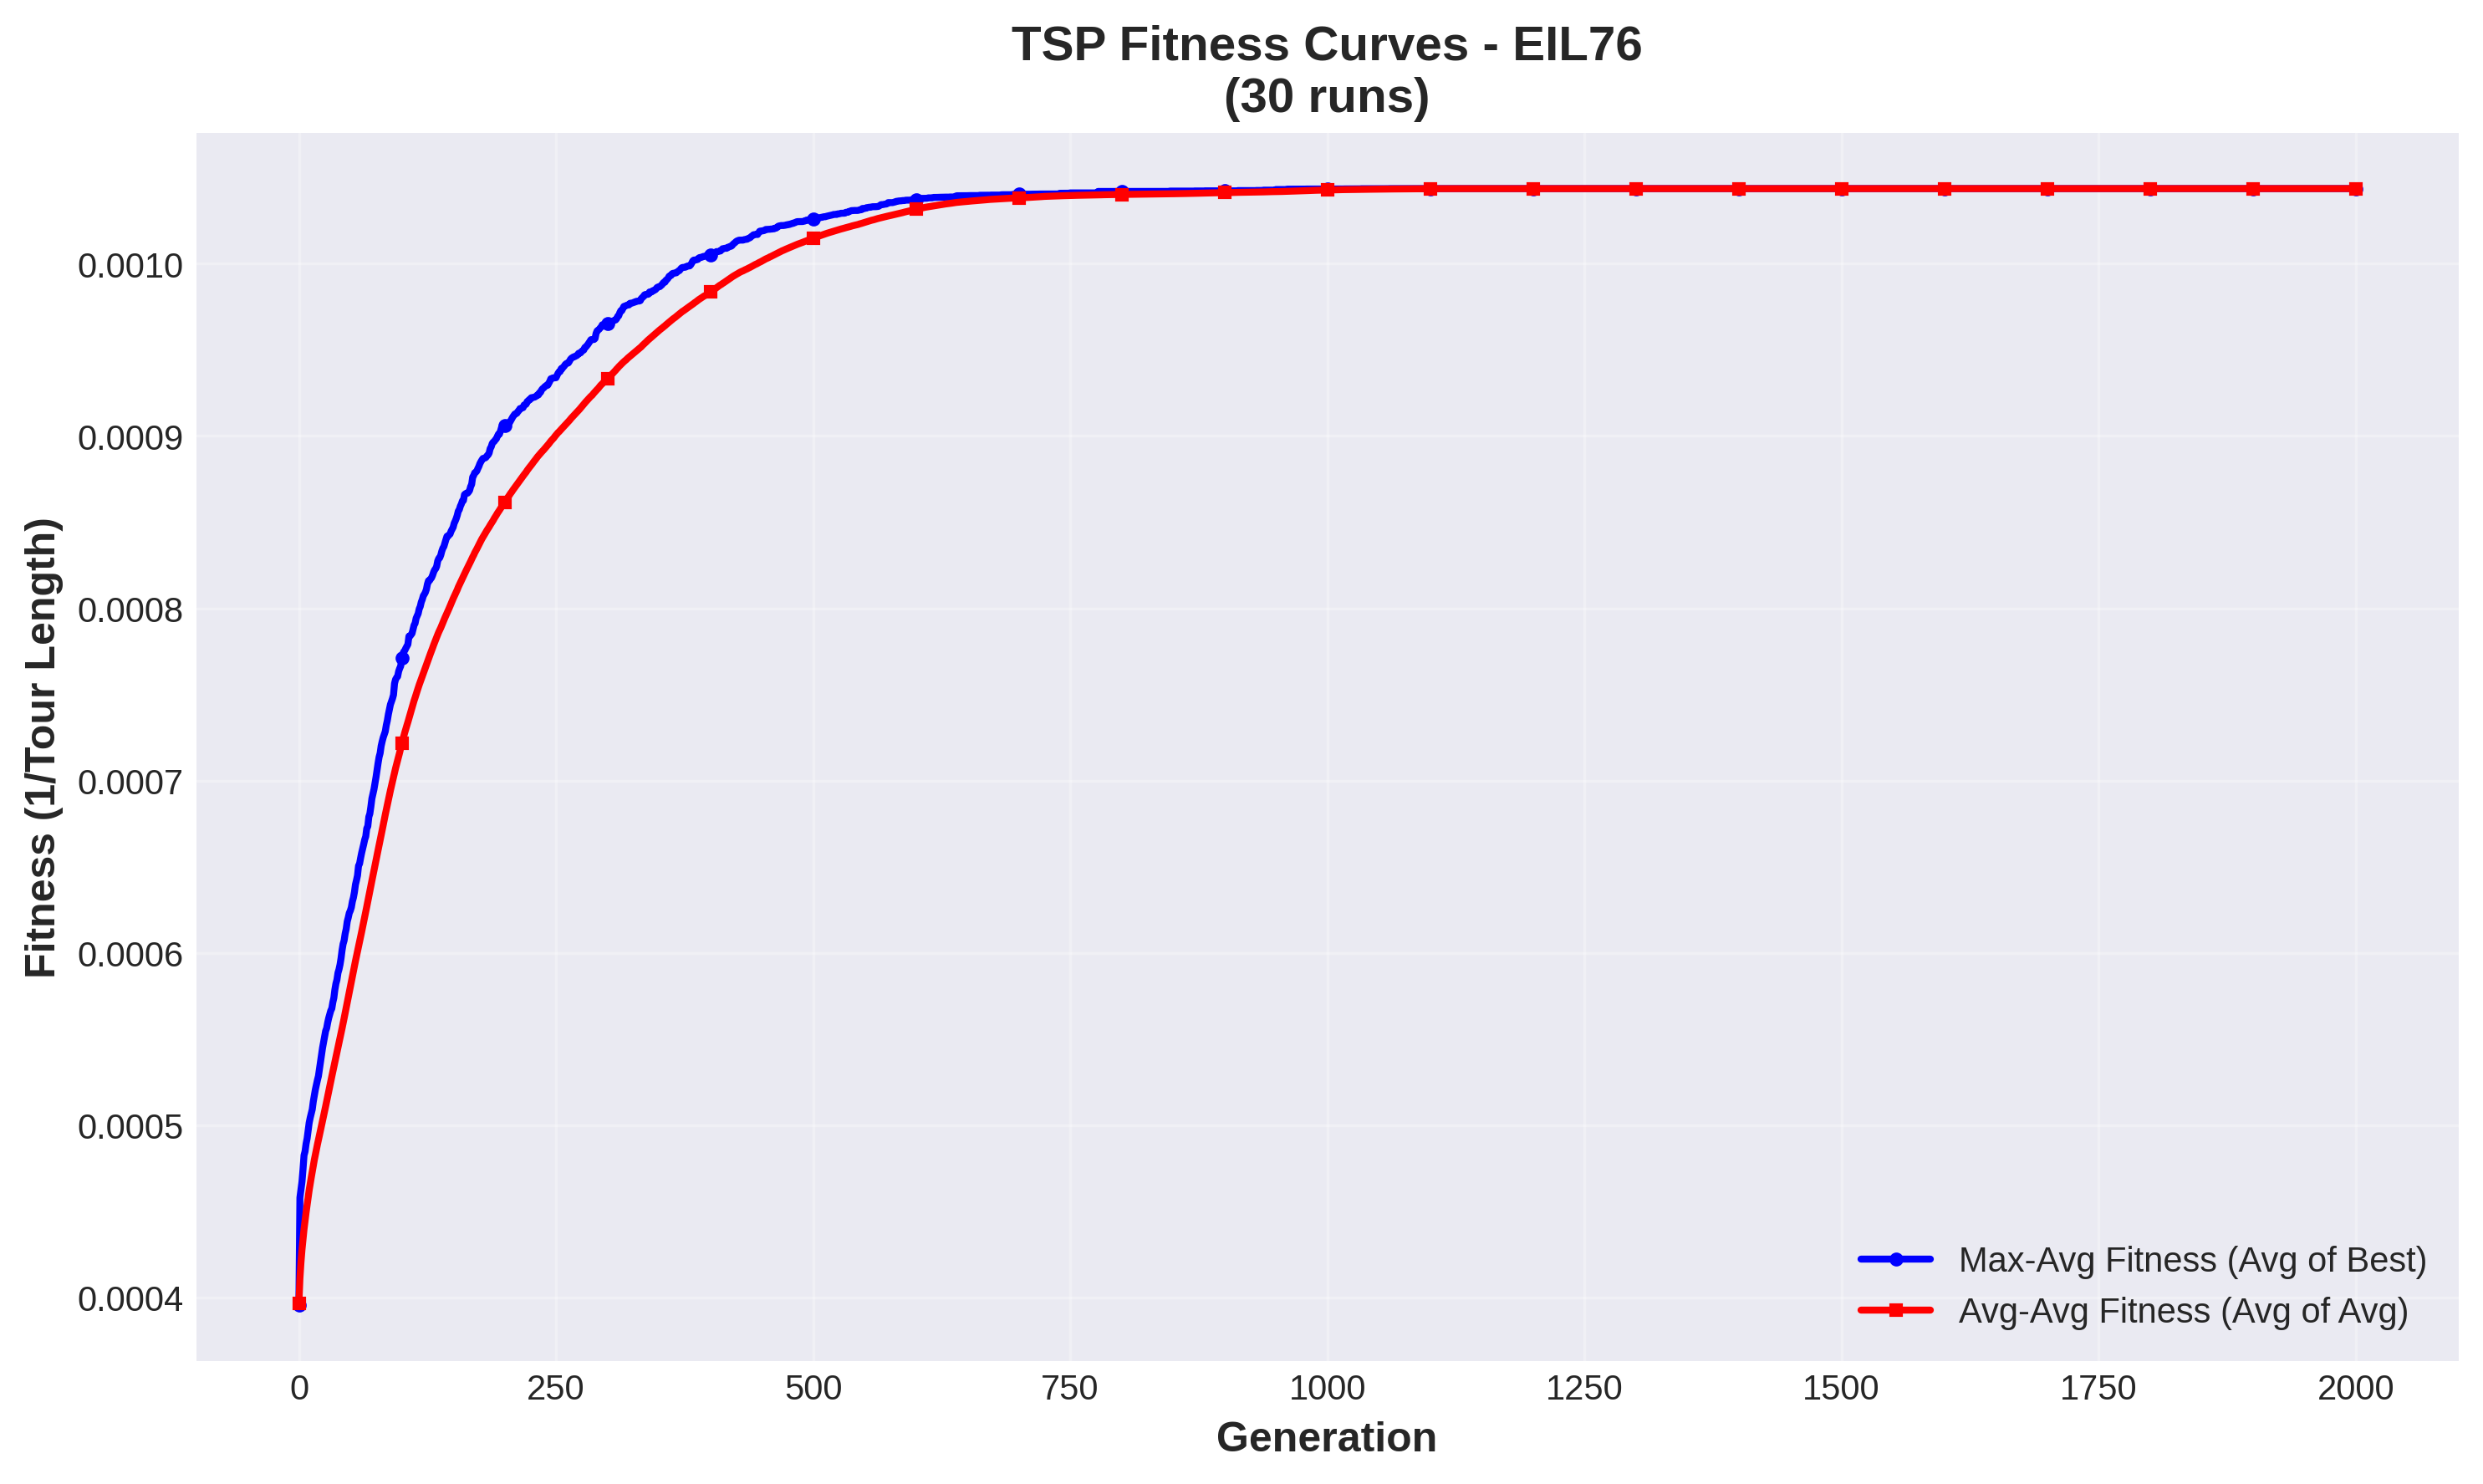
\includegraphics[width=0.8\textwidth]{eil76_fitness_curves.png}
    \caption{Fitness curves for \texttt{eil76} (R$\ge$30).}
\end{figure}

\begin{figure}[H]
    \centering
    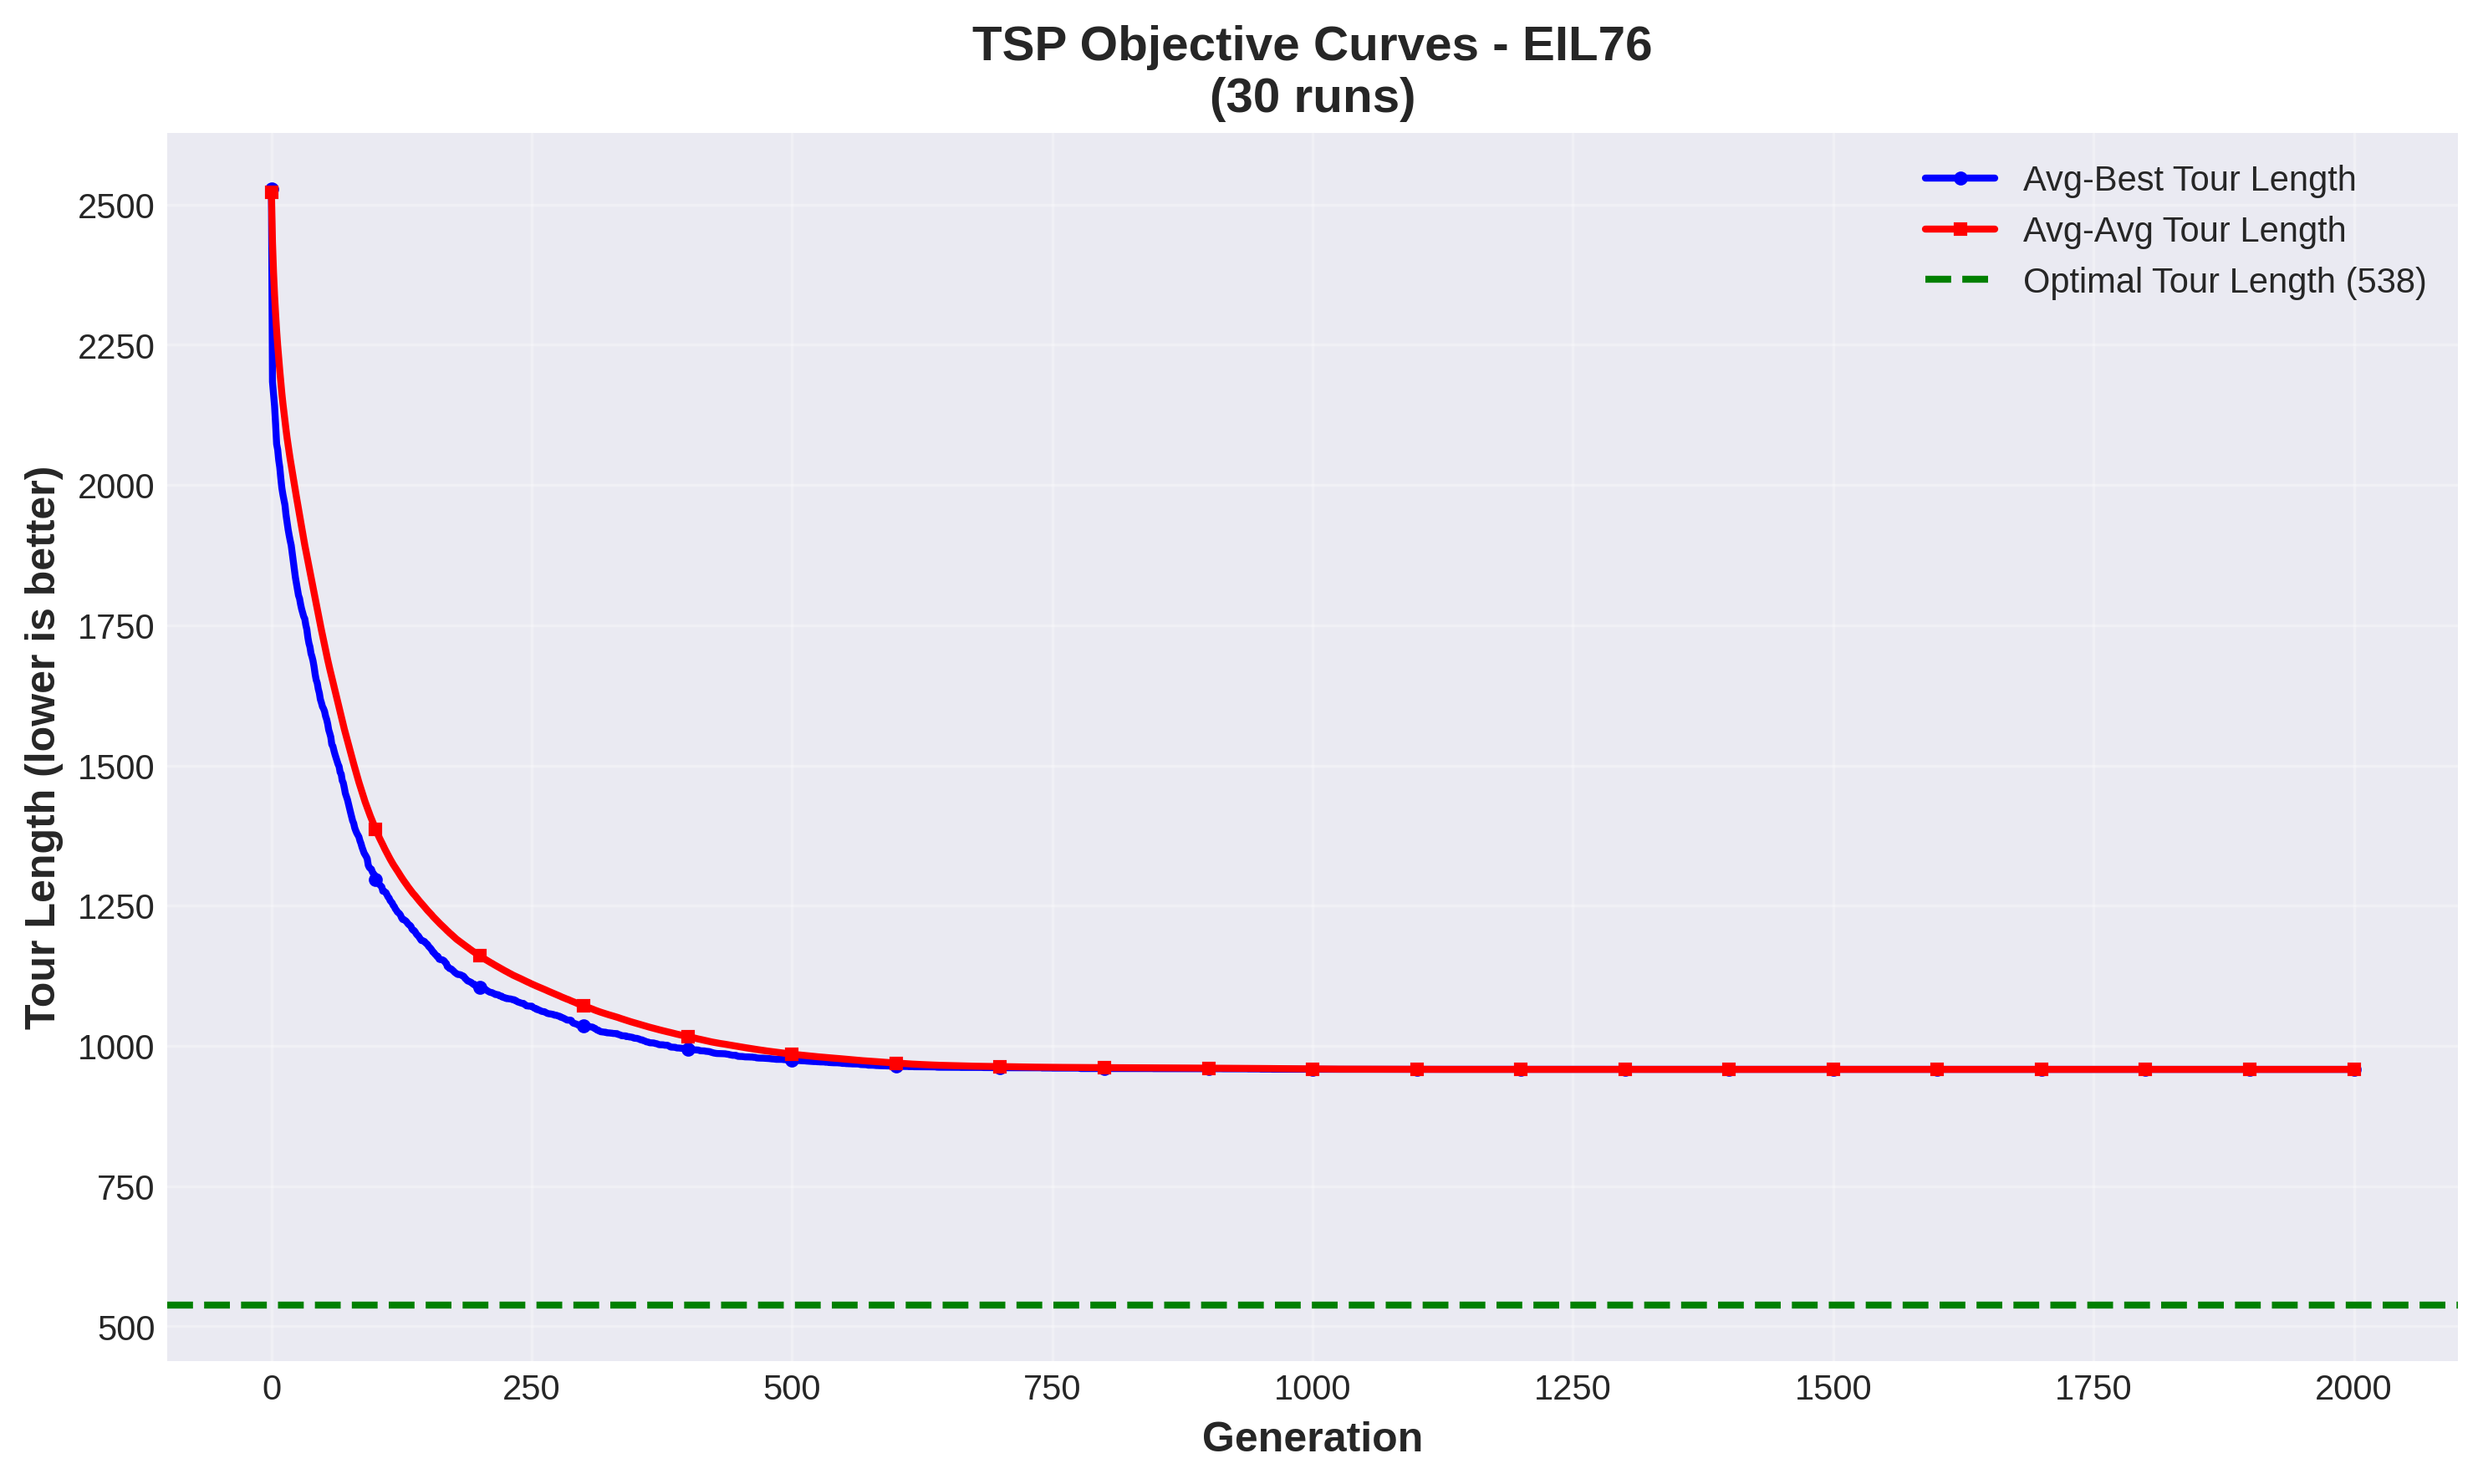
\includegraphics[width=0.8\textwidth]{eil76_objective_curves.png}
    \caption{Tour length curves for \texttt{eil76} (R$\ge$30).}
\end{figure}

\clearpage

\begin{figure}[H]
    \centering
    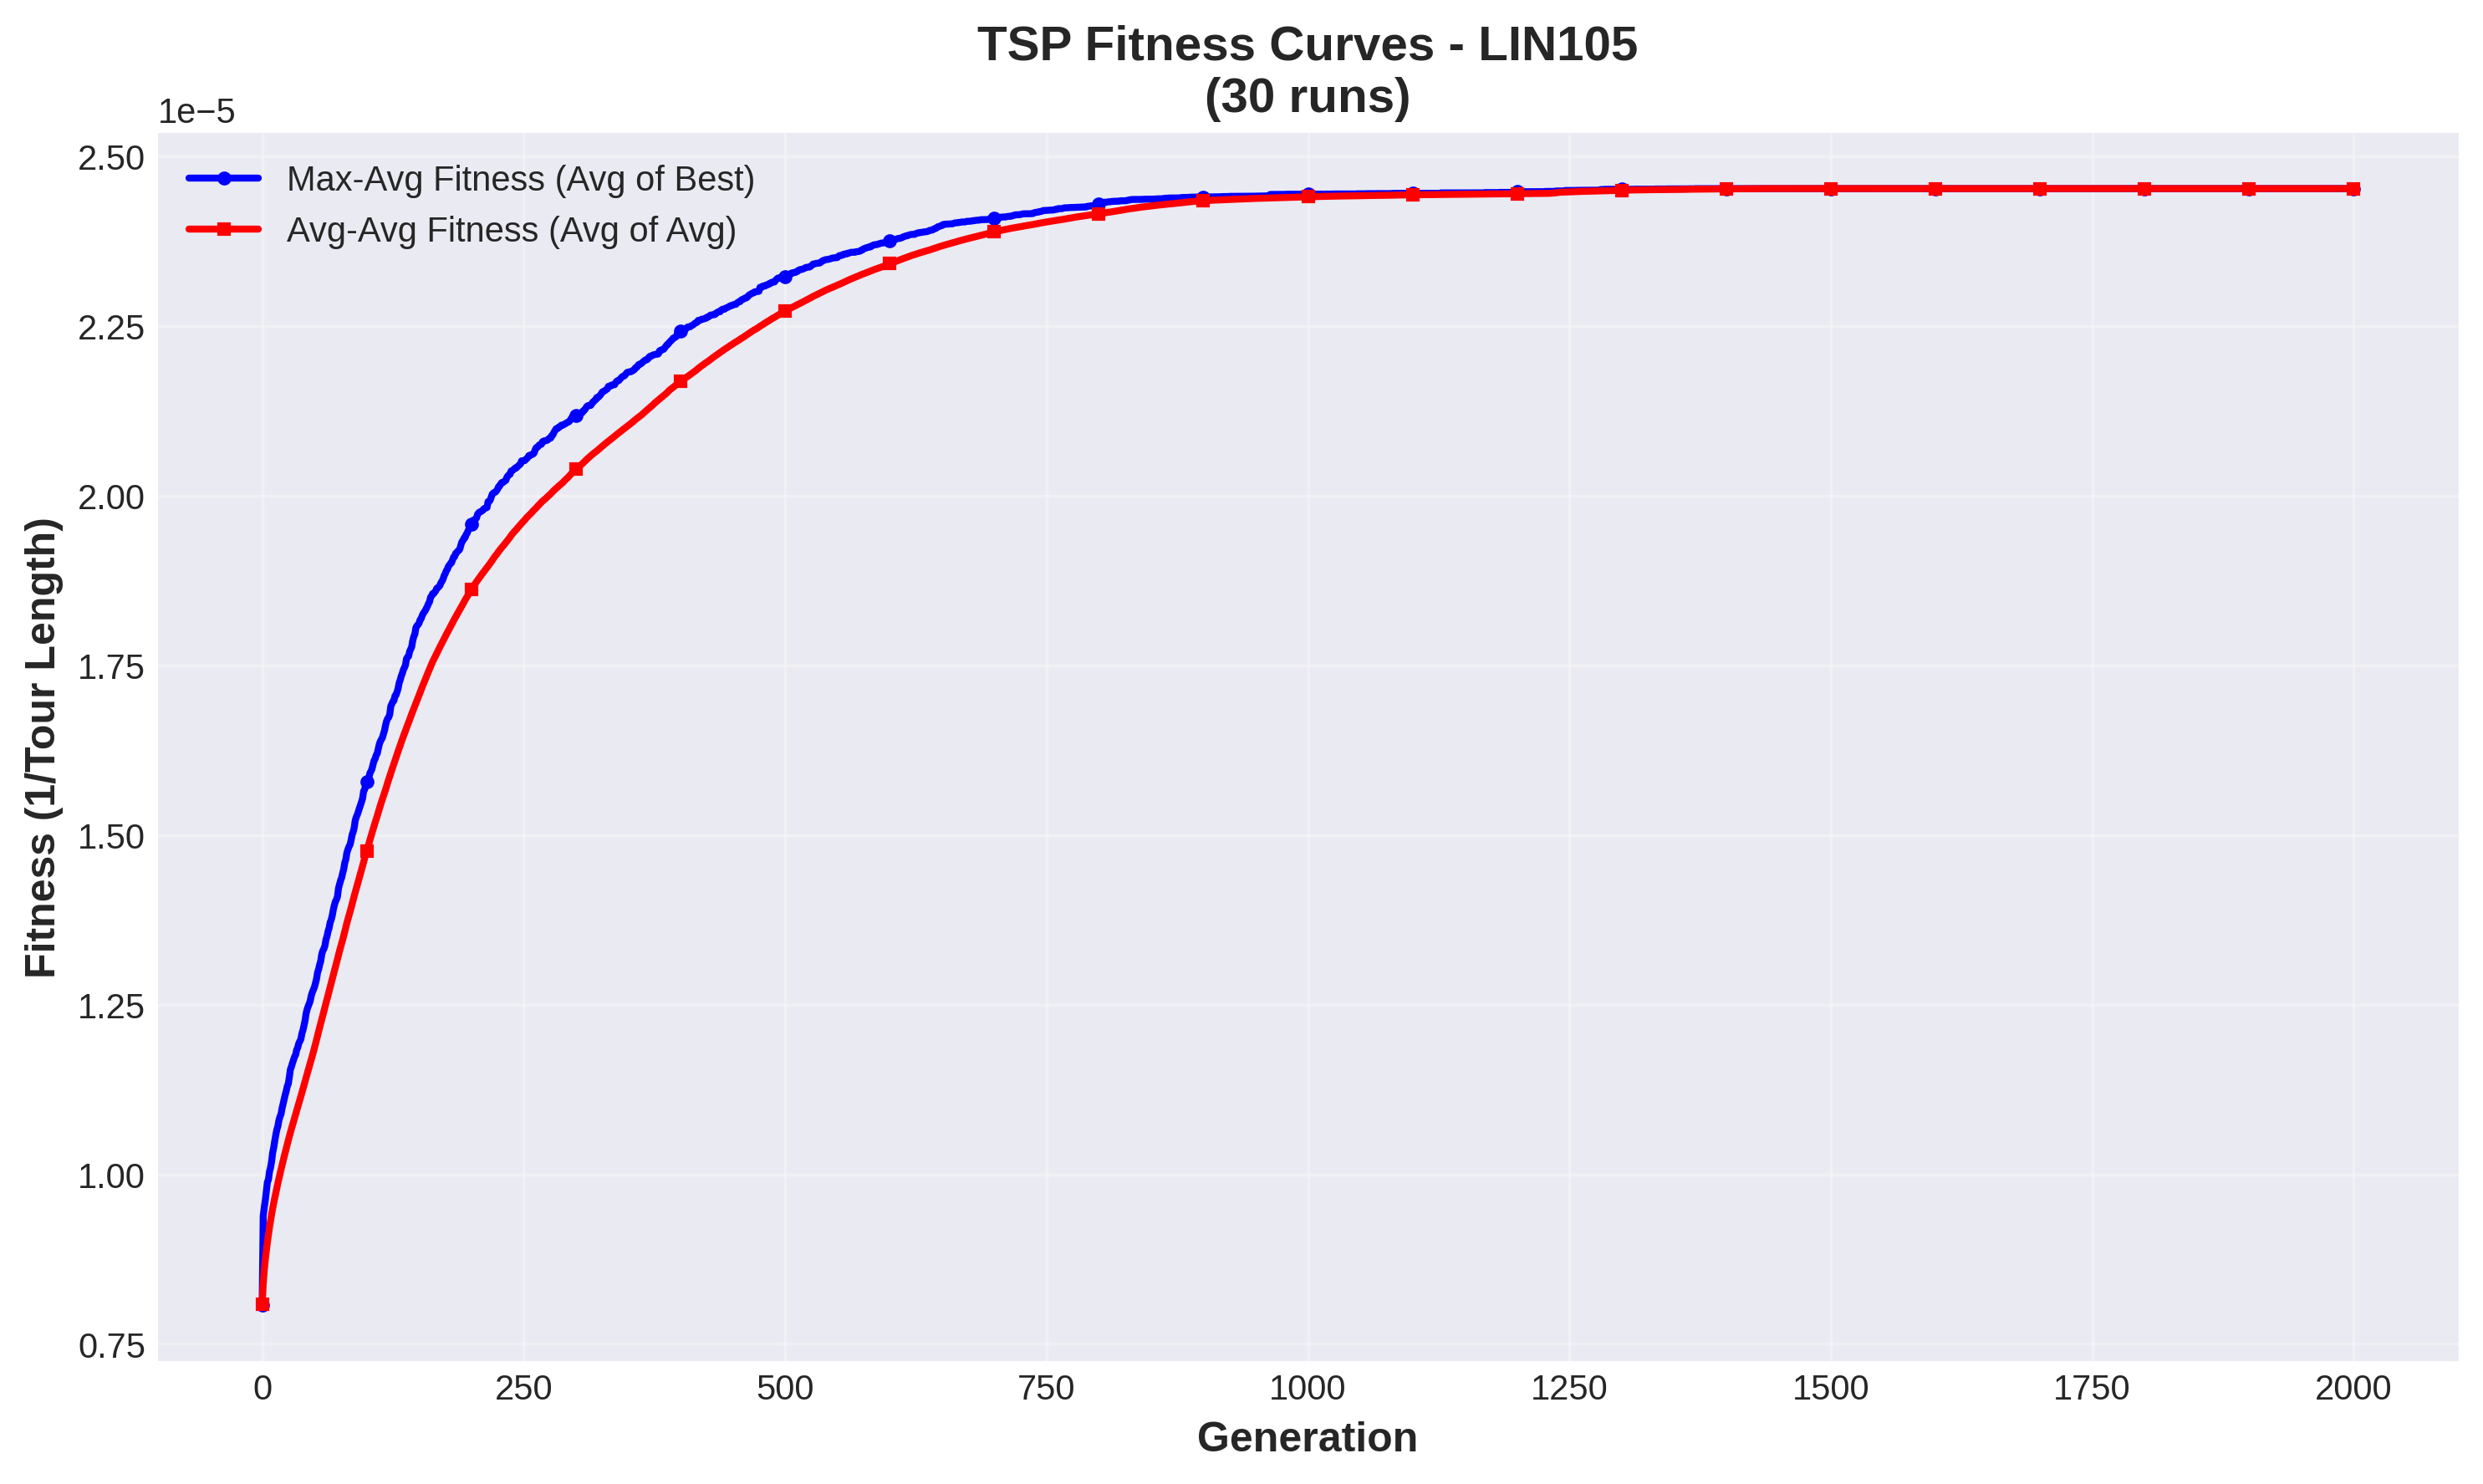
\includegraphics[width=0.8\textwidth]{lin105_fitness_curves.png}
    \caption{Fitness curves for \texttt{lin105} (R$\ge$30).}
\end{figure}

\begin{figure}[H]
    \centering
    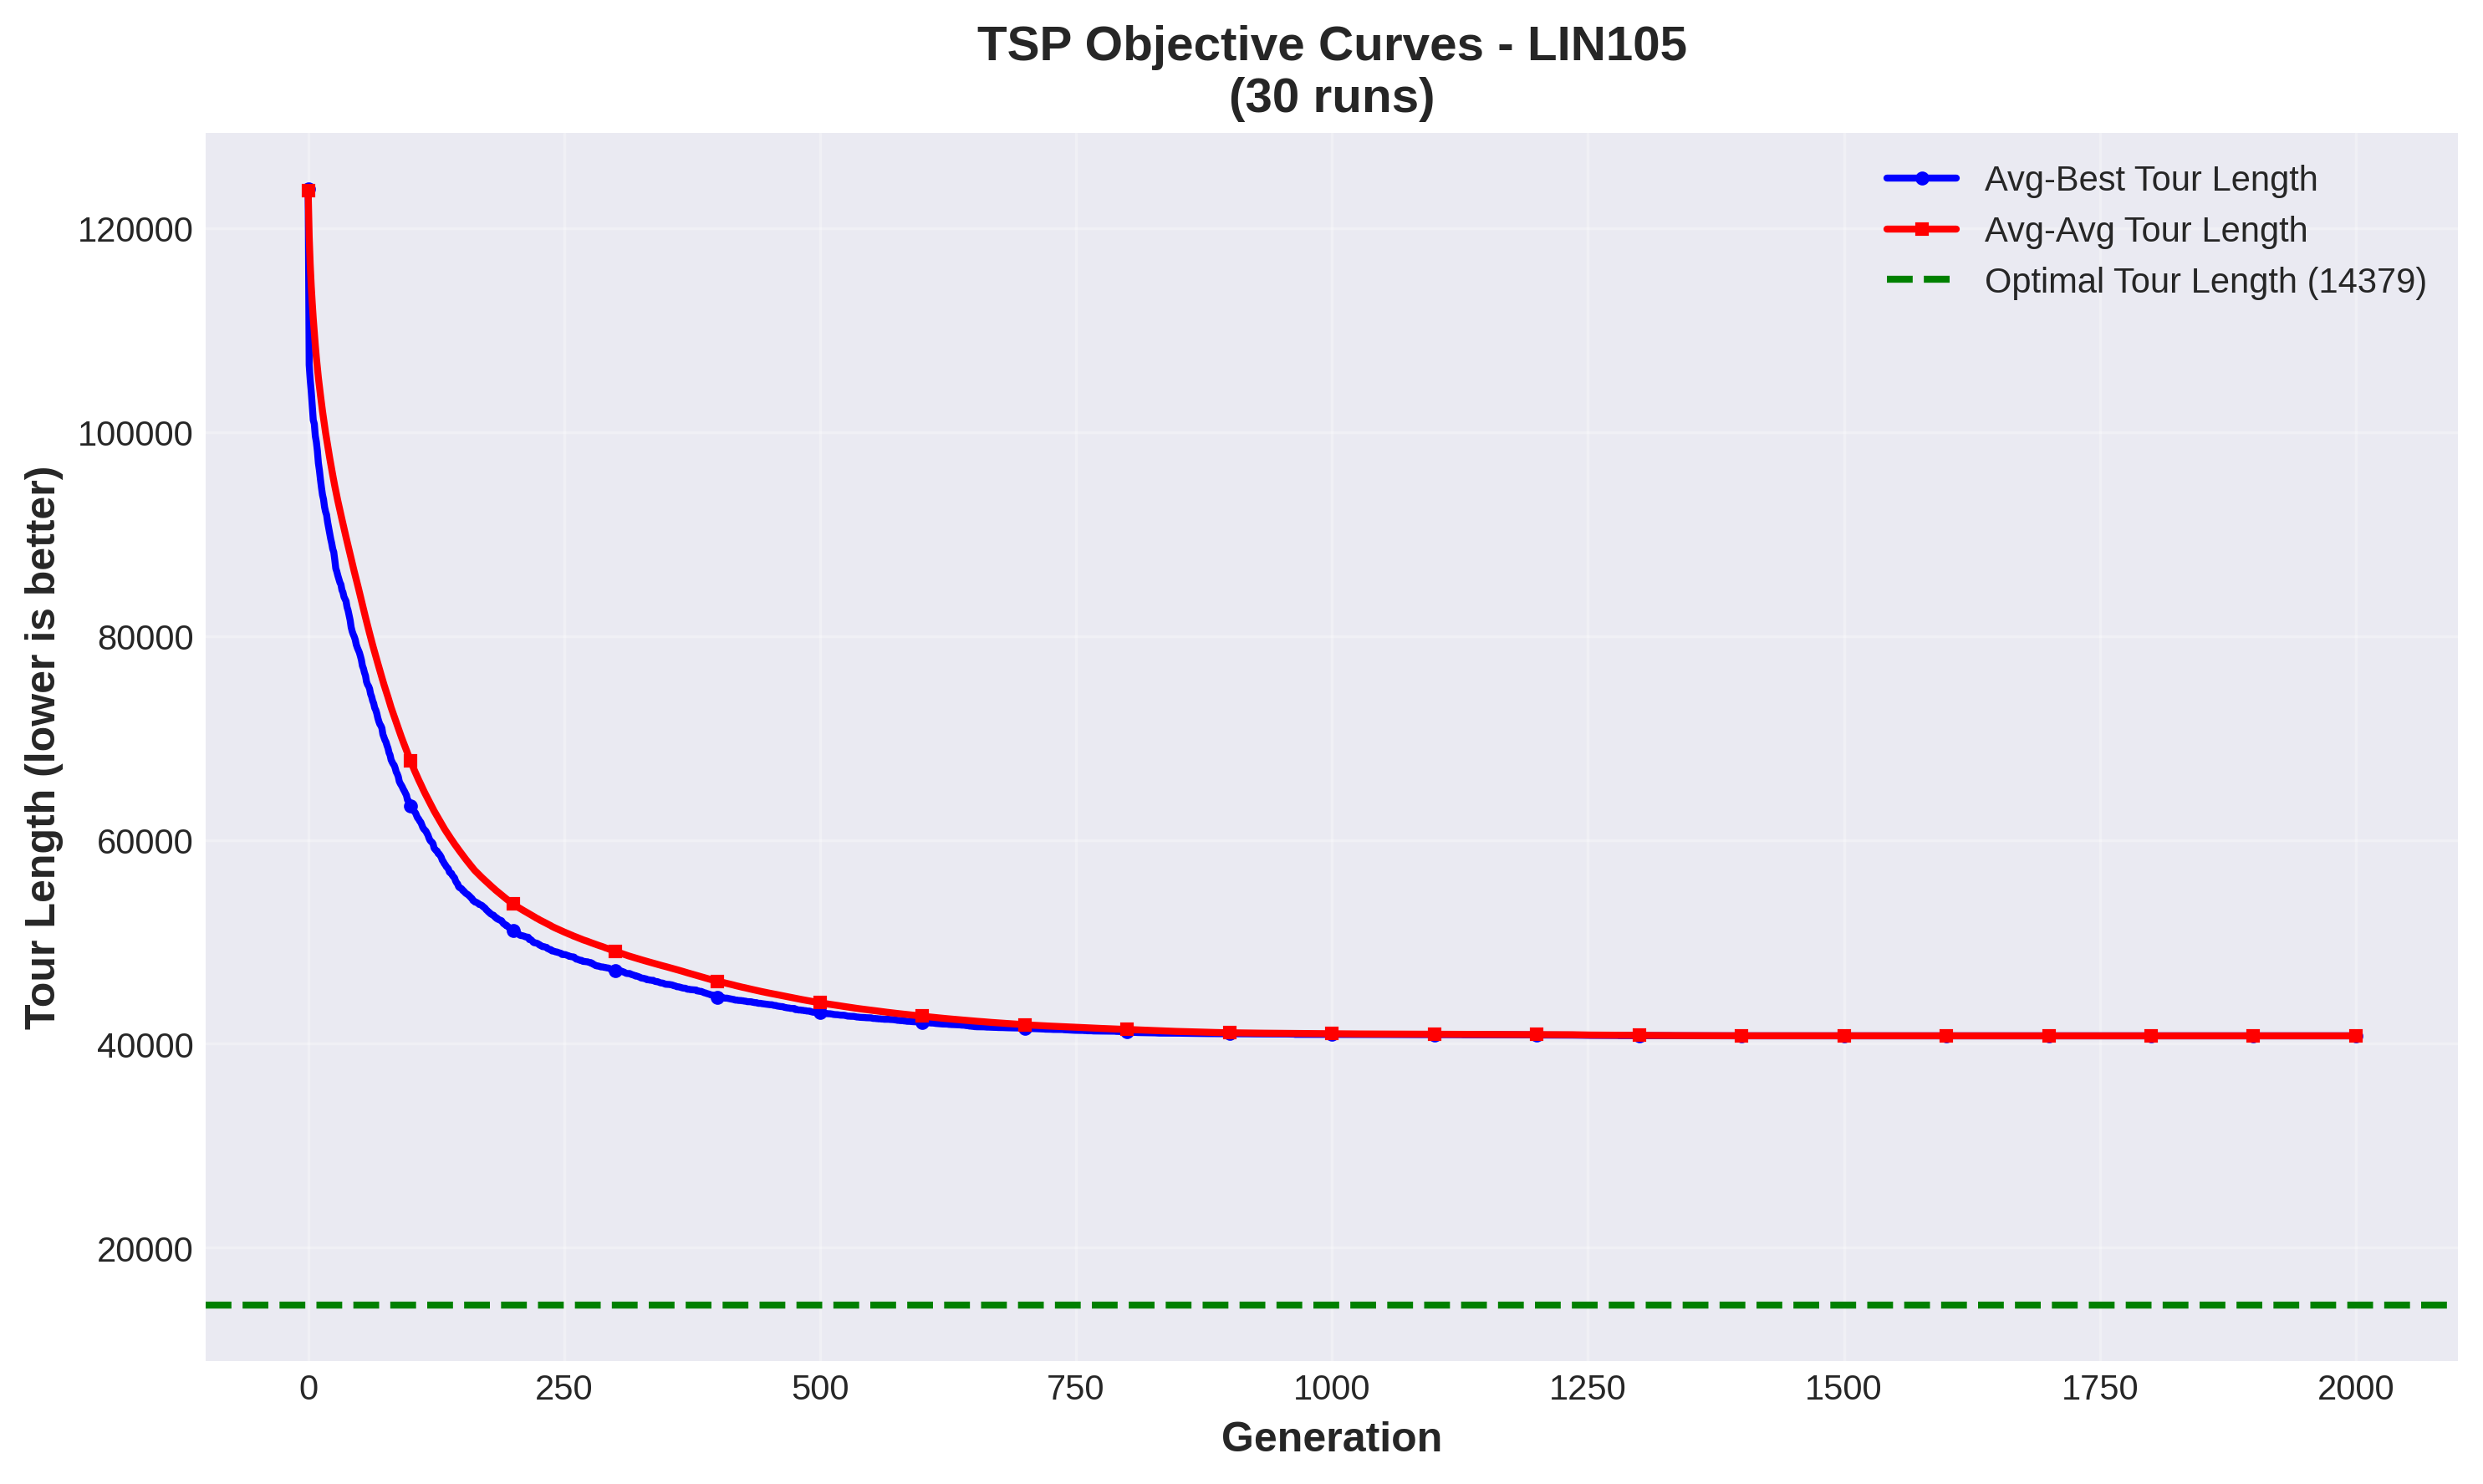
\includegraphics[width=0.8\textwidth]{lin105_objective_curves.png}
    \caption{Tour length curves for \texttt{lin105} (R$\ge$30).}
\end{figure}

\clearpage

\begin{figure}[H]
    \centering
    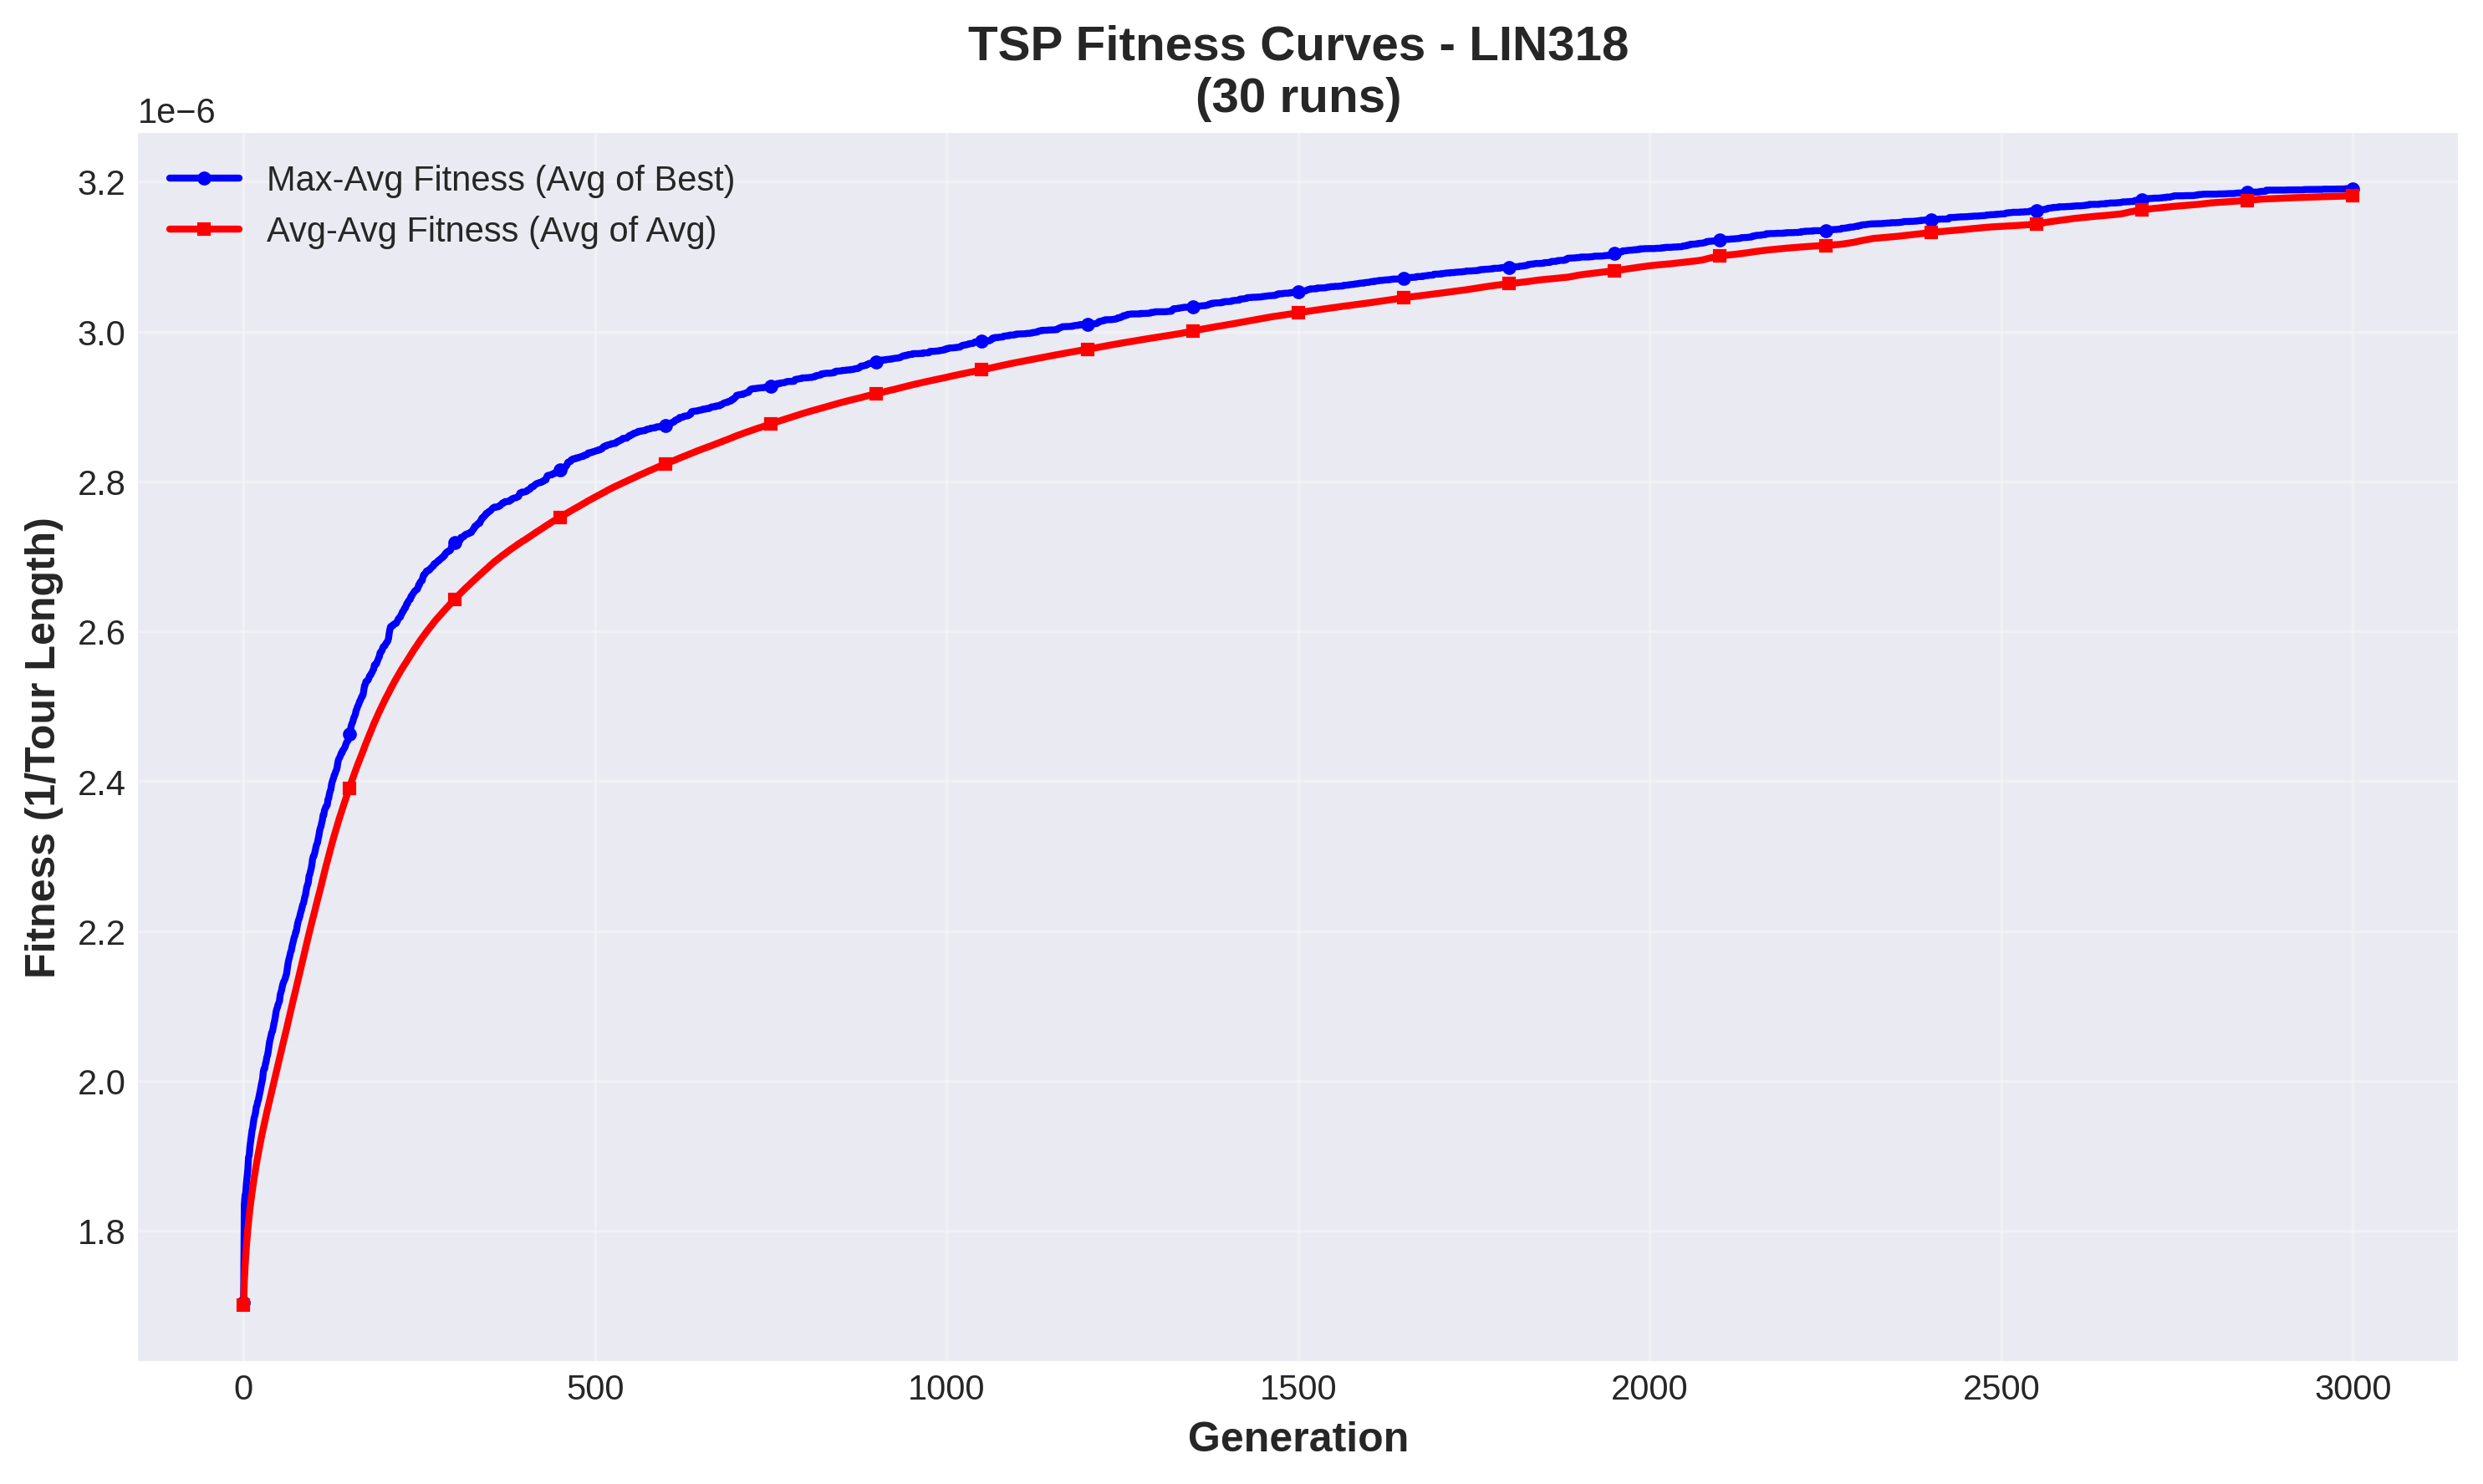
\includegraphics[width=0.8\textwidth]{lin318_fitness_curves.png}
    \caption{Fitness curves for \texttt{lin318} (R$\ge$30).}
\end{figure}

\begin{figure}[H]
    \centering
    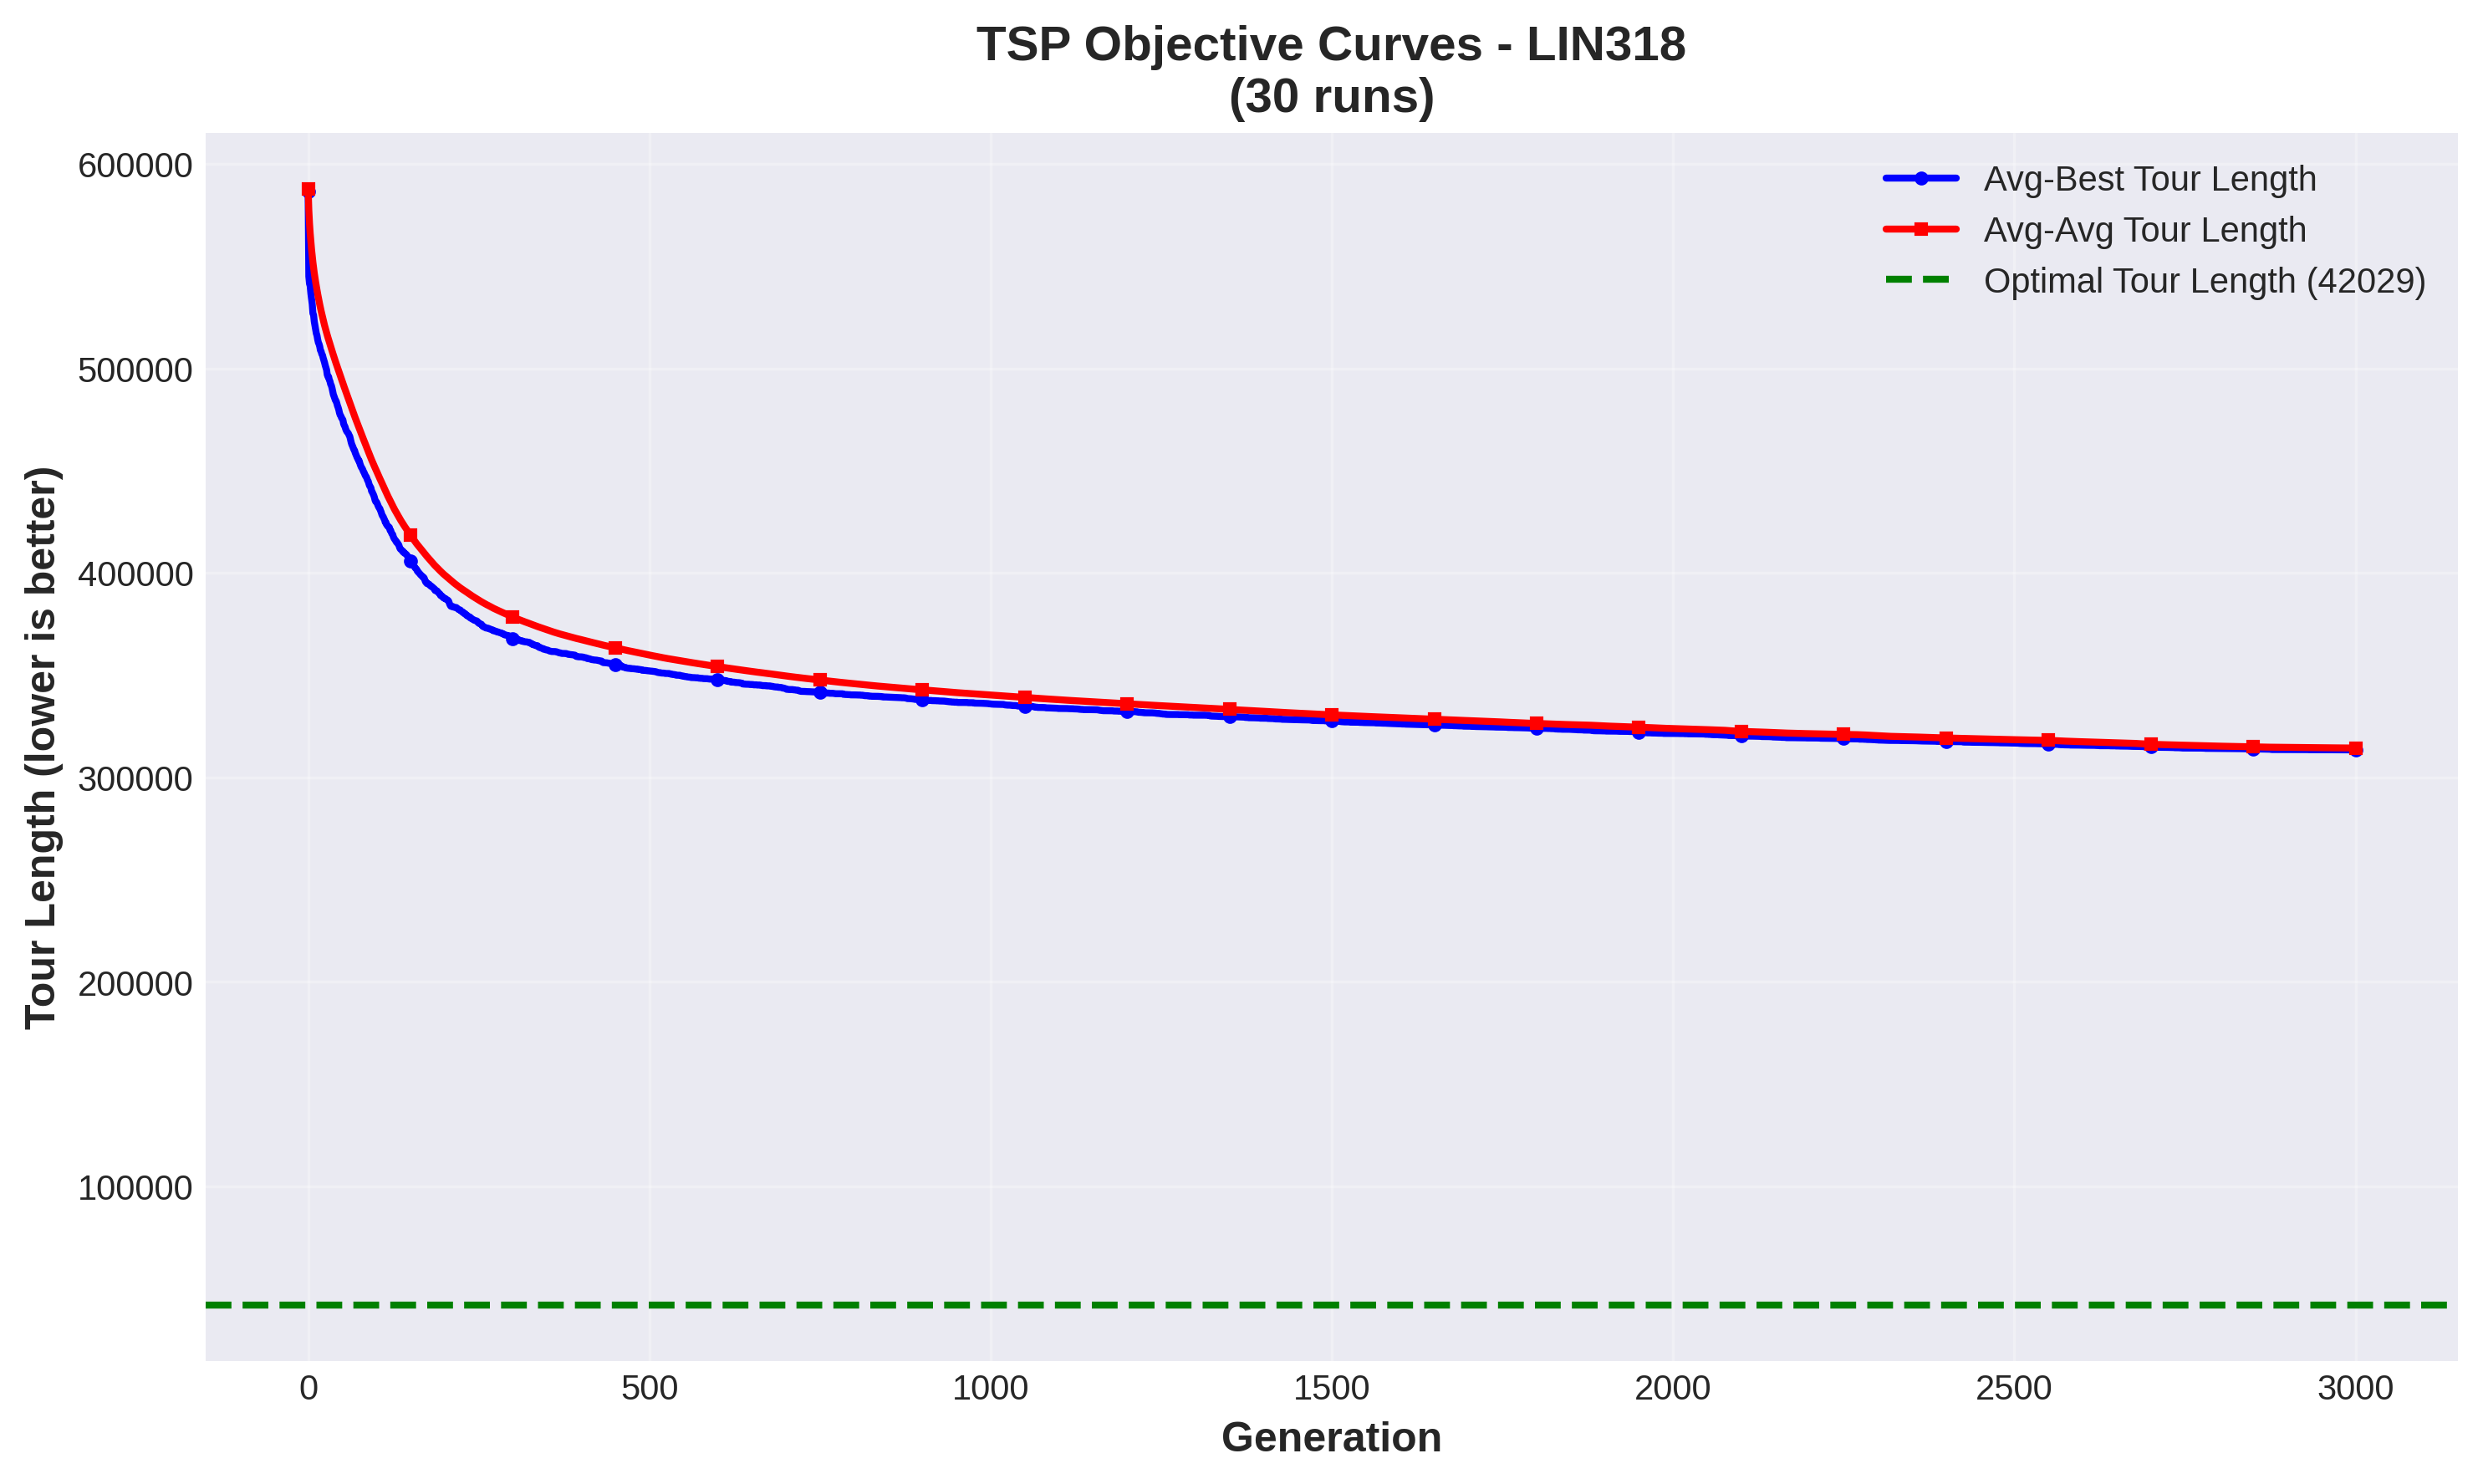
\includegraphics[width=0.8\textwidth]{lin318_objective_curves.png}
    \caption{Tour length curves for \texttt{lin318} (R$\ge$30).}
\end{figure}

\subsection{Discussion}
A permutation-only GA with PMX stalls without local search. CHC’s threshold and cataclysms help diversity but do not enforce edge structure. The effective recipe is \emph{edge-aware recombination + local search}. PMX is serviceable; OX/ERX often preserve edges better; with 2-Opt, the difference narrows. To push closer to OPT on larger sets: (i) use a memetic GA (2-Opted offspring each generation), (ii) maintain selection pressure via rank-based/shifted fitness \cite{potvin1996gaTSP,johnson1997tspLocal,nagata2013eax}.

\subsection{What counts as ``Speed''}
We define Speed as mean evaluations (over seeds) to reach the Quality threshold (the GA’s mean Quality per instance). For stricter auditing, a fixed bar (e.g., $\le 10\%$ over OPT) can also be reported.

\section{References}
\begin{thebibliography}{99}

\bibitem{goldberg1989ga}
D.~E.~Goldberg.
\newblock \emph{Genetic Algorithms in Search, Optimization, and Machine Learning}.
\newblock Addison--Wesley, 1989.

\bibitem{eshelman1991chc}
L.~J.~Eshelman.
\newblock The CHC adaptive search algorithm: How to have safe search when engaging in nontraditional genetic recombination.
\newblock In \emph{Foundations of Genetic Algorithms}, pages 265--283. Morgan Kaufmann, 1991.

\bibitem{goldberg1985pmx}
D.~E.~Goldberg and R.~Lingle.
\newblock Alleles, loci, and the traveling salesman problem.
\newblock In \emph{Proceedings of the First International Conference on Genetic Algorithms}, pages 154--159, 1985.

\bibitem{oliver1987ox}
I.~M.~Oliver, D.~J.~Smith, and J.~R.~C.~Holland.
\newblock A study of permutation crossover operators on the traveling salesman problem.
\newblock In \emph{Proceedings of the Second International Conference on Genetic Algorithms}, pages 224--230, 1987.

\bibitem{lin1973lk}
S.~Lin and B.~W.~Kernighan.
\newblock An effective heuristic algorithm for the traveling-salesman problem.
\newblock \emph{Operations Research}, 21(2):498--516, 1973.

\bibitem{potvin1996gaTSP}
J.-Y.~Potvin.
\newblock Genetic algorithms for the traveling salesman problem.
\newblock \emph{Annals of Operations Research}, 63:337--370, 1996.

\bibitem{reinelt1991tsplib}
G.~Reinelt.
\newblock TSPLIB---A traveling salesman problem library.
\newblock \emph{ORSA Journal on Computing}, 3(4):376--384, 1991.

\bibitem{johnson1997tspLocal}
D.~S.~Johnson and L.~A.~McGeoch.
\newblock The traveling salesman problem: A case study in local optimization.
\newblock In E.~H.~L. Aarts and J.~K. Lenstra (eds.), \emph{Local Search in Combinatorial Optimization}, pages 215--310. Wiley, 1997.

\bibitem{nagata2013eax}
Y.~Nagata and S.~Kobayashi.
\newblock A powerful genetic algorithm using edge assembly crossover for the traveling salesman problem.
\newblock \emph{INFORMS Journal on Computing}, 25(2):346--363, 2013.

\bibitem{murata1996sequencepair}
H.~Murata, K.~Fujiyoshi, S.~Nakatake, and Y.~Kajitani.
\newblock VLSI module placement based on rectangle-packing by the sequence-pair.
\newblock \emph{IEEE Transactions on Computer-Aided Design of Integrated Circuits and Systems}, 15(12):1518--1524, 1996.

\bibitem{chang2000bstar}
Y.-W.~Chang, Y.-W.~Chang, G.-C.~Chen, and S.-C.~Wu.
\newblock B$^\ast$-Trees: A new representation for non-slicing floorplans.
\newblock In \emph{Proceedings of the 37th Design Automation Conference (DAC)}, pages 458--463, 2000.

\bibitem{moscato1999ma}
P.~Moscato.
\newblock Memetic algorithms: A short introduction.
\newblock In \emph{New Ideas in Optimization}, pages 219--234. McGraw-Hill, 1999.

\end{thebibliography}

\end{document}